\documentclass[../main.tex]{subfiles}

\begin{document}

\chapter{Modèle discret pour le criblage haut-débit du potentiel d'interaction métabolique dans les écosystèmes microbiens complexes}
\label{ccmc}
\minitoc
Article en cours de rédaction 
%\textit{journal theory of biology}. \footnote{\url{https://www.sciencedirect.com/journal/journal-of-theoretical-biology}}

%\doublespacing %% For correction

\newpage

\section{Introduction}
Dans le chapitre précédent, nous avons développé une approche itérative permettant de prédire des concentrations de métabolites, la densité bactérienne ainsi que quelques interactions bactériennes dans un écosystème composé de 3 souches bactériennes. Cette approche est numériquement trop coûteuse en temps pour permettre une analyse haut-débit d'écosystèmes microbiens plus complexes. De plus, la prédiction des interactions bactériennes a été faite avec confiance grâce à la connaissance \textit{a priori} des biologistes, de la littérature et des données expérimentales. Dans le cadre d'un écosystème naturel, appliquer le processus itératif décrit dans le chapitre \ref{tango} est compromis par le manque de la connaissances \textit{a priori} du système. En effet, raffiner des modèles métaboliques appartenant à des organismes peu étudiés et générer des données de calibration pour des communautés composées de centaines d'espèces sont irréalisables. \\

La stabilité des communautés microbiennes se reposent en partie sur les interactions bactérie-bactérie, principalement caractérisées par la consommation et la production de métabolites. Ces interactions sont particulièrement importantes car elles sont responsables du fonctionnement du microbiome: protection de l'hôte dans le microbiote de l'intestin \citep{WILMES20221201}, recyclage de matières organique dans le sol \citep{Rousk2016}, participation à la croissance de la plante \citep{FOURNIER202227} ou encore, ou développement d'arôme dans la fermentation du fromage \citep{Cao2021}. Pour rappel, il existe plusieurs types d'interaction comme illustré par la Figure \ref{fig:interaction}. La coopération est déterminée comme un échange métabolique positif, sans effet négatif pour la bactérie productrice et la receveuse. A l'opposé, la compétition est décrite comme un coe-consommation d'un substrat limitant impactant la croissance et /ou la production métabolique des bactéries en compétition.\\

Dans la littérature, nous avons observé que les méthodes pour identifier des potentiels de coopération et de compétition dans des communautés de grande taille s'intéressaient à l'étude du métabolisme (voir chapitre \ref{ch:edla}). En effet, en utilisant la relation d'association gène-protéine-réaction d'un réseau métabolique à l'échelle du génome (GEM), une représentation sous forme d'une matrice st\oe{}chiométrique, d'un graphe ou à l'aide d'approches de raisonnement peuvent être utilisé pour mettre en avant ces interactions. Comme nous l'avons vu, les approches numériques sont principalement limitées par le coût calculatoire. Les approches basées sur les graphes ne sont pas non plus adaptées à la caractérisation de ces potentiels d'interactions lorsque que le nombre d'organisme dans la communauté est important. En effet, des approches se basent sur des analyses par paire d'organismes, rendant fastidieuse l'analyse à l'échelle de la communauté. Il existe cependant un compromis, permettant de caractériser la communauté dans son ensemble, comme les méthodes numériques, et permettant de passer à l'échelle de grandes communautés: \textbf{l'approche par raisonnement} \citep{Belcour.2020, Frioux2018}. Au moyen d'un formalisme logique, des règles décrivant la notion de productibilité d'un composé sont décrites (voir chapitre \ref{EDLA}). \\

Pour caractériser les potentiels d'interactions à l'aide de l'approche par raisonnement, une base de connaissance décrivant l'objet d'étude sous forme d'une liste de faits biologiques doit être créée. Dans notre cas, elle est constituée des attributs d'un réseau métabolique que sont: produit, réactant, réaction, métabolite. Cette base de connaissance va permettre d'analyser rapidement la productibilité des composés, la faisabilité des réactions ou encore, d'identifier les échanges métaboliques etc. Toutes ces propriétés émergeantes sont calculables à partir d'une liste de règles inspirées des définitions biologiques décrivant ces mêmes particularités. Ainsi, chaque modèle en sortie découlera explicitement de la règle biologique auditable. Le paradigme de programmation par ensemble de réponse (de l’\textit{anglais, Answer set Programming} ou ASP) a été choisi pour ses qualités: explicabilité des modèles et résolution des problèmes combinatoires.\\

Dans ce chapitre, nous avons donc utilisé la programmation par ensemble de réponse (ASP) et s'inspiré de l'algorithme d'expansion du réseau métabolique d'Ebenhoh \citep{Ebenhoh2004} et de son élargissement à la caractérisation de communauté \citep{Frioux2018} en créant une nouvelle base de connaissance à partir d'un ensemble de GEMs. De cette base de faits, des nouvelles règles logiques sont créées permettant le calcul d'un potentiel de coopération et de compétition. Dans la suite, nous présenterons la nouvelle base de connaissance et les règles logiques que nous avons développées, puis une série de tests montrant la pertinence des scores de coopération et de compétition. Enfin, une comparaison à des méthodes quantitatives sera effectuée. \\

Les travaux présentés dans ce chapitre ont mené à un article en cours de rédaction et à plusieurs posters scientifiques et présentations orales \citep{lecomte:hal-03839337,lecomte:hal-03857781, lecomte:hal-03857848}

%pour une soumission dans \textit{journal of theory biology} \footnote{\url{https://www.sciencedirect.com/journal/journal-of-theoretical-biology}}

\newpage
\section{Méthode pour calculer un score d'interaction à partir d'une base de connaissance}
Le choix de la représentation de la connaissance est primordial pour toute approche par raisonnement. Nous détaillerons dans un premier temps, comment nous avons représenté mathématiquement et en ASP la base de faits, ainsi que les règles logiques pour inférer les potentiels d'interaction.

\subsection{Base de faits d’un réseau métabolique}
À partir de la donnée d'entrée, un GEM, nous avons défini des ensembles de réactions \Rs, métabolites \Ms et de taxa \Ts où taxon représente l'identifiant du GEM. Nous avons associé chaque ensemble de métabolites \Ms et réactions \Rs à son taxon \Ts et récupéré le nom ontologique donné dans le GEM $\name$ comme suit:

\begin{align}
	\begin{split}
		& \source: \Ms \rightarrow \Ts \\
		& \source: \Rs \rightarrow \Ts \\
		& \name: \Ms \rightarrow \mbox{\textit{identifiant}}
	\end{split} 
\end{align}

L'association d'un métabolite ou d'une réaction à son taxon permet d'obtenir la réaction ou le métabolite à partir d'un ensemble de taxa:

\[\projection{t\in\Ts} = \{ m \in M \suchthat \source(m) = t \}\]

Nous avons par la suite défini les relations entre les métabolites, réactions et taxon sous la représentation d'un graphe bipartite. Pour rappel, une réaction est composée d'un ensemble de réactant et de produit, et nous le formalisons de la façon suivante:

\begin{align}
\begin{split}
    \products(\gmodel) &= \{ m\in M \suchthat \langle r, m\rangle \in E \} \\
    \reactants(\gmodel) &= \{ m\in M \suchthat \langle m, r\rangle \in E \} \\
    \taxons(M) & = \{ t \in T \suchthat \exists m\in M ,\, \source(m) = t \}
\end{split}
\end{align}

dans lequel, \gmodel est le tuple défini par $\langle M, R, E \rangle$, $r \in \Rs$; où chaque arc $e = \langle m,r \rangle$ encode un \emph{réactant} consommé par la réaction $r$ et $e = \langle r,m \rangle$ encode un \emph{produit} produit de $r$. \\

Tout comme pour le modèle numérique, un choix concernant la prise en compte des réactions de transport présentes dans le réseau métabolique a été fait. Il a été montré que le phénomène de lyse cellulaire était une potentielle source d'interaction métabolique, entrainant la mort de la cellule et libérant son contenu métabolique dans le milieu extracellulaire \citep{Fazzino2020}. De plus, \citep{Pacheco.2019m3q} ont montré que les sécrétions passives étaient une source de mutualisme au sein de communautés bactériennes. De ce fait, lors de la conception du modèle de communauté, nous avons choisi de considérer les ensembles de métabolites produits en intracellulaire disponibles pour tous. Ainsi, un modèle de Communauté \( \gcommunity = \{ \gmodel[1], ..., \gmodel[n] \}\) peut-être décrit comme le produit cartésien de l'union des métabolites et réactions défini par le graphe bipartite, et se lit ainsi:

\[
\merge(\gcommunity) = 
\left\langle \bigcup^{n}_{i=1} M_i, \bigcup^{n}_{i=1} R_i, \bigcup^{n}_{i=1} E_i \right\rangle \,.
\]

\subsection{Productibilité d'un métabolite}
Pour rappel, un métabolite $mp$ est productible si l'ensemble des réactants d'une réaction, permettant la production de ce métabolite $mp$, sont disponibles à partir d'un ensemble de graines, constitué de l'ensemble des composés du milieu nutritif. Dans la suite de ce chapitre, nous qualifierons de \emph{scope} l'ensemble des métabolites productibles par un réseau à partir de graines. Du fait de notre représentation de la base de connaissance, dans lequel chacun des métabolites et réactions est associé à un GEM, nous n'avons plus la nécessité de distinguer le \emph{scope} associé à un individu de celui de la communauté comme dans \citep{Frioux2018}. Ainsi, à partir d'un ensemble de graines $S$ et pour une communauté de GEMs $\gmodel$, le \emph{scope} est défini comme suit:

\[
\begin{split}
    \scope(\gcommunity,S) & = \bigcup^{\infty}_{i=0} \scope_i \mbox{, où} \\
    \scope_0 & = S\\
    \scope_{i+1} & = \scope_i \bigcup \products(\{ r \in R \suchthat \\ 
     & \name(\reactants(r)) \subseteq \name(\scope_i) \}) \,.
\end{split}
\]

Pour implémenter cette notion de productibilité et calculer des potentiels de coopération et de compétition, nous avons utilisé une approche par raisonnement.

\subsection{L'inférence des règles logiques pour calculer les potentiels de coopération et de compétition}
Cette sous-section présentera comment nous avons implémenté en ASP les définitions de \texttt{scope}, de coopération et de compétition.

\paragraph*{Inférence du scope métabolique.} 
A partir d'un objet métabolite, dans lequel un nom et un taxon sont associés, (\texttt{metabolite(M,B)}) et d'une communauté (\texttt{Communaute}), le \texttt{scope} métabolique d'une communauté est défini par le code \ref{lst:scope} et \ref{lst:disponible}. Dans la suite de cette section, chaque listing sera expliqué ligne par ligne sous forme d'item, afin de comprendre les règles logiques. 

\begin{lstlisting}[mathescape=True,label={lst:scope},caption={Code ASP permettant de calculer le scope métabolique}, captionpos=b]
scope(metabolite(M,B), Communaute) :- taxon(B);  
               in_community(Communaute,B); 
               reaction(R,B); product(M,R,B); 
               disponible(M', Communaute) : reactant(M',R,B).
\end{lstlisting}

Au sein du listing \ref{lst:scope}, un métabolite est dans le scope d'une communauté si :
\begin{itemize}
	\item[ligne 1:] le \texttt{scope} métabolique, d'une communauté est vrai si, \texttt{B} est un taxon et
	\item[ligne 2:] que \texttt{B} est un membre de la communauté et
	\item[ligne 3:] qu'il existe une réaction \texttt{R} du taxon \texttt{B} qui produit \texttt{M} et 
	\item[ligne 4:] que tous les métabolites réactants de la réactant \texttt{R} du taxon \texttt{B} sont disponibles pour la communauté.\\
\end{itemize}

De cette règle découle la notion de disponibilité d'un métabolite (voir listing \ref{lst:disponible})

\begin{lstlisting}[mathescape=True, label={lst:disponible}, caption={Code ASP permettant de savoir si un métabolite est disponible},captionpos=b]
disponible(M,Com) :- graine(M), Communaute(Com). 
disponible(M,Com) :- scope(metabolite(M,B), Com).
\end{lstlisting}

où :

\begin{itemize}
	\item[ligne 1:] Un métabolite \texttt{M} est disponible pour une communauté \texttt{Com} si le métabolite M est une graine et que \texttt{Com}  est une communauté de GEMs où
	\item[ligne 2:] que le métabolite \texttt{M} appartenant à un taxon \texttt{B} est dans le \texttt{scope} métabolique de la communauté \texttt{Com}. 
\end{itemize}

\paragraph*{Inférence des métabolites échangeable.} Nous avons pris le postulat que les métabolites échangés correspondent à l'approximation la plus directe de la coopération d'une communauté. Nous l'avons défini comme un métabolite qui est productible par un GEM, consommable par un autre et qui ne peut être produit par ce dernier:

\[
\begin{split}
\exchange_{\gcommunity, S}(\hat{m}) = \{ \langle P, C \rangle \suchthat &
         \exists \gmodel[C]\in\gcommunity,
         \exists \gmodel[P]\in\gcommunity, \\
    &    \exists m \in \reactants(\gmodel[C]), \\
    & \name(m) = \hat{m}, \\
    & m \in \products(\gmodel[P]), \\
    & m \not\in \scope(\gmodel[C],S), \\
    & m \in \projection{P}(\scope(\gcommunity, S)) \;\} \\
\end{split}
\]
dans lequel $S$ correspond au \texttt{scope} métabolique, $P$ et $C$ respectivement les taxa producteur et consommateur.

Le code ASP correspondant est similaire à sa représentation mathématique et est défini par le code \ref{lst:echange}:
\begin{lstlisting}[mathescape=True, label={lst:echange}, caption={Code ASP permettant d'obtenir l'ensemble des métabolites qui sont potentiellement échangés.}, captionpos=b]
exchange(M,P,C) :- taxon(P), 
		 taxon(C),
		 P != C,
		 reactant(M,_,C),
		 product(M,_,P),
		 scope(metabolite(M,P), all),
		 not scope(metabolite(M,C), self(C)).
\end{lstlisting}

où:

\begin{itemize}
	\item[ligne 1:] un métabolite \texttt{M} est échangeable entre un producteur \texttt{P} et un consommateur \texttt{C} si \texttt{P} est un taxon et 
	\item[ligne 2:] que \texttt{C} est un taxon et
	\item[ligne 3:] \texttt{P} est différent de \texttt{C} et
	\item[ligne 4:] que \texttt{M} est un réactant de n'importe quelle réaction de \texttt{C} et 
	\item[ligne 5:] que \texttt{M} est un produit de n'importe quelle réaction de \texttt{P} et
	\item[ligne 6:] que \texttt{M} est dans le \texttt{scope} communautaire et 
	\item[ligne 7:] que \texttt{M} n'est pas dans le \texttt{scope} de \texttt{C}.
\end{itemize}

Nous avons décrit le \texttt{scope} métabolique pour un GEM ou une communauté de GEMs, et identifié les métabolites échangeables comme un proxy de la coopération. Concernant la compétition, la notion de substrat limitant est reliée à la quantité de ressource de ce substrat  disponible pour la communauté. Ce formalisme discret ne permet actuellement pas de prendre la notion de quantité, nous nous sommes inspirés d'un concept d'économie pour définir une compétition: polyopsonie. D'origine grec, l'éthymologie de monopsone appliqué à l'économie signifie un marché dans lequel il y a un seul acheteur (\textit{mono} signifie un, et \textit{opsonia}  signifie achat). Un marché où il existe un petit nombre d'acheteur est charactérisé par l'oligopsone. En s'inspirant des deux concepts economiques ci-dessus, nous avons élaboré un nouveau mot représentant un marché où il existe plusieurs acheteurs: polyopsone.


\paragraph*{Inférence de la polyopsonie.} Ainsi, la polyopsonie reflète une approximation de la compétition et stipule que les substrats limitants, \textit{i.e.} métabolites échangeables et ceux qui sont consommés par plus d'un organisme, sont considérés comme substrats en compétition. Mathématiquement, cela se traduit par:

\begin{align}
	\begin{split}
	\lims(\gcommunity,& S) = \{ \name(m) \suchthat
     	\exists m\in \reactants(\scope(\gcommunity, S)), \\
    	& \vert \taxons(m) \vert > 1 \;\wedge \\
    	& (\name(m) \in S \vee 
      	\exchange_{\gcommunity,S}(\name(m)) \neq\emptyset) \;\} \, . \\
	\end{split}
\end{align}
dans lequel $m$ est un métabolite. \\
%
%
%Littéralement, cette expression signifie que pour chaque métabolite $m$ considéré comme réactant dans le scope ($m\in \reactants(\scope(\gcommunity, S))$) et est consommé par au moins 2 individus ($\vert \taxons(m) \vert > 1$) et qu'il est échangeable ($\exchange_{\gcommunity,S}(\name(m)) \neq\emptyset) \;\} $) alors, nous le considérons comme limitant. \\

Dans le code mathématique ci-dessus, le facteur déterminant un substrat limitant concerne le nombre de taxa consommant un métabolite. Ainsi, dans le code ASP permettant d'obtenir les substrats qui sont limitants (voir listing \ref{lst:competition}), nous avons compté le nombre de taxa consommant chaque substrat, échangé ou considéré comme un nutriment, et appliqué la condition du nombre de consommateur:

\begin{lstlisting}[mathescape=True,label={lst:competition}, caption={Code ASP permettant d'obtenir l'ensemble des consommateurs en compétition pour un substrat limitant.}, captionpos=b]
% cas pour les metabolites echangeables
polyopsonist(M,N) :- N=#count{C,M:exchange(M,_,C)},
		 	exchange(M,_,_), N > 1.
		 	
% cas pour les graines
polyopsonist(S,N) :- N=#count{B:seed_consumed_by_taxon(S,B)}, 
			N > 1, seed(S).
\end{lstlisting}

où :

\begin{itemize}
	\item[ligne 2-3:] Un composé échangé \texttt{M} est limitant si lorsque le nombre de consommateurs \texttt{C} impliqués dans l'échange de ce métabolite \texttt{M} est strictement supérieur à 1.
	\item[ligne 6-7:] Une graine \texttt{M} est considérée limitante lorsque le nombre de consommateur s\texttt{C} de cette graine \texttt{M} est strictement supérieur à 1. \\
\end{itemize}

Les codes ASP que nous avons décrit correspondent à des règles qui sont biologiquement explicables et génèrent un vocabulaire contrôlé (par cet ensemble de règles). Dans les sections suivantes seront montrés comment à partir de ce vocabulaire nous avons calculé les scores de potentiels de coopération et de compétition. 

\subsection{Calcul des potentiels de coopération et de compétition à partir des règles logiques}
Ces scores ont pour objectif de comparer des communautés d'une taille comparable entre elles et de pouvoir les classer de la plus coopérative à la plus compétitive. Nous les avons donc façonnés pour qu'ils puissent être robustes à différentes perturbations. Deux tests de robustesses ont été faits: modification du milieu nutritionnel et taxonomique. 

Nous verrons tout d'abord comment ces scores ont été créés.

\paragraph*{Calcul du potentiel de coopération}
L'inférence de la coopération se base sur les taxa impliqués dans l'échange d'un métabolite (voir listing \ref{lst:echange}). Pour chaque métabolite échangeable, nous avons un ensemble non nul de consommateurs et de producteurs. L'ensemble des producteurs (resp. consommateurs), notés $\textsf{P}(\hat{m})$ (resp. $\textsf{C}(\hat{m})$) associé à chaque métabolite échangé $\hat{m}$ est calculé de la façon suivante:

\begin{align}
\begin{split}
    \textsf{P}(\hat{m}) & =
        \{ t\in \Ts \suchthat \langle t, C \rangle \in \exchange_{\gcommunity, S}(\hat{m}) \} \\
    \textsf{C}(\hat{m}) & =
        \{ t\in \Ts \suchthat \langle P, t \rangle \in \exchange_{\gcommunity, S}(\hat{m}) \} \,. 
\end{split}
\end{align}



À partir de ces ensembles, identifier les taxa réellement producteurs et consommateurs nécessite l'ajout de connaissances \textit{a priori}. Désirant être applicable à n'importe quel écosystème et sans ajout de connaissances, nous avons supposé que chacun des taxa producteurs (resp. consommateurs) contribue à l'échange. Une contribution égale de chaque taxon producteurs (resp. consommateur), c'est à dire que chaque taxon peut produire (resp. consommer) le métabolite échangé, surestimerait la coopération. À l'inverse, supposer qu'un seul taxon parmi les producteurs (resp. consommateurs) contribue à l'échange, sous-estimerait la coopération. \\

Lors d'un échange métabolique, un producteur ne peut pas fournir le composé échangé à l'ensemble des consommateurs. Un compromis équitable a donc été fait stipulant que chaque taxa producteur (resp. consommateur) peut produire (resp. consommer) le métabolite échangé, mais la contribution des taxa n'est pas égale. Ainsi, pour chaque métabolite échangeable, le compromis équitable consiste à attribuer un poids $w$ de 1 au premier producteur (resp. consommateur) de l'ensemble $\textsf{P}(\hat{m})$ (resp. $\textsf{C}(\hat{m})$), puis d'ajouter un bonus exponentiel dégressif pour chacun des producteurs (resp. consommateurs) restant. Formellement, ce poids $w$ s'écrit:

\[
w(k) = \sum_{i=0}^k 2^{-i}
\]

 dans lequel $i$ correspond à l'index d'un producteur (resp. consommateur). Il est important de noter que nous ne prétendons pas que $2^{-i}$ est le coefficient optimal pour analyser des communautés. Cette valeur permet de ne pas surestimer ou sous-estimer la coopération en attribuant tout de même une contribution pour chaque organisme. De plus, ce poids a permis à la fois de pénaliser la redondance de producteurs (resp. consommateurs) pour chaque nouveau métabolite échangeable, et à la fois suppose qu'un métabolite échangé n'est pas obligatoirement disponible pour l'ensemble des individus. \\
 
 
 Enfin, le score final consiste à sommer les contributions pour chaque métabolite échangé obtenu avec le poids:
 
 \begin{align}
\label{coop}
    \textsf{CooP} = \sum\limits_{\hat{m}\in\Ms}
                    w(\vert\textsf{P}(\hat{m})\vert) + 
                    w(\vert\textsf{C}(\hat{m})\vert) \,.
 \end{align}

À partir du calcul \ref{coop}, nous pouvons déduire la contribution des producteurs et des consommateurs dans le score de coopération final, en calculant:

\[
\begin{split}
    \textsf{CooP\raisebox{-0.4ex}{-}producers} & = \sum\limits_{\hat{m}\in\Ms} w(\vert\textsf{P}(\hat{m})\vert) \\
    \textsf{CooP\raisebox{-0.4ex}{-}consumers} & = \sum\limits_{\hat{m}\in\Ms} w(\vert\textsf{C}(\hat{m})\vert)
\end{split}
\]

\paragraph*{Calcul du score de compétition.}
L'inférence de la compétition se base sur le nombre de consommateurs de substrats limitants. Le potentiel de compétition se calcul en considérant l'ensemble des consommateurs de tous les substrats polyopsonistes, divisé par la taille de la communauté. Ainsi, pour une communauté $\gcommunity$ et un scope $S$, le score de compétition est défini par: 

\[
    \textsf{ComP} = \frac{\vert\lims(\gcommunity,S)\vert}{\vert \gcommunity \vert} \,.
\]


\subsection{Expériences \textit{in silico} pour tester différentes propriétés des scores}
Afin de tester ces scores, nous avons généré des communautés artificielles et calculé les scores de coopération et de compétition à partir de l'inférence logique. Puis, nous les avons comparés avec différents outils sur différents jeux de données. La sous-section suivante explique la provenance des données ainsi que les différents tests effectués.

\paragraph*{Données et génération de communautés synthétiques}
Nous avons collecté les génomes appartenant à différents écosystèmes: 857 du sol de la base de données RefSoil \cite{Choi2017}, 1520 du microbiote humain \cite{Zou2019}, 186 de la racine d'\textit{Arabisopsis thaliana} ((PRJNA297942) et 189 de la feuille (PRJNA297956) d'\textit{Arabisopsis thaliana} \cite{Bai2015}. Nous avons effectué une annotation structurale et fonctionnelle par Prodigal \cite{Hyatt2010} v.2.6.3 et eggNOG-mapper \cite{Cantalapiedra2021} v.2.1.6 sur la base de données the eggNOG \cite{Huerta-Cepas2019} v.5.0.2. Nous avons reconstruit les réseaux métaboliques à l'échelle du génome en utilisant Pathway-Tools v.25.5 \cite{Karp2022} et mpwt v.0.7 \cite{Belcour.2020}. Nous avons ensuite constitué 2 types de milieux de culture: 1 générique où les macros et micro-nutriments standards sont présents, et 1 spécifique de chaque écosystème. Ces milieux sont disponibles dans l'annexe \ref{graine-specific-generic}.

A partir de ces données, nous avons créé des communautés artificielles pour chaque écosystème. Ainsi, pour l'intestin, la feuille, la racine et le sol, 50 communautés de taille 5, 10, 20, 30, 50, 75, 100 et 150 ont été générées aléatoirement. Nous avons en plus créé une communauté factice, noté \textit{mixte} dans le reste du chapitre, composé des différents réseaux métaboliques de chaque écosystème pour les mêmes tailles de communautés et dans des proportions égales. \\

Afin de vérifier si la structure du réseau à une importance dans les scores des potentiels d'interaction, nous avons testé la similarité des réseaux métaboliques deux à deux, vérifiant la corrélation entre les scores obtenus et la topologie réactionnelle du réseau métabolique. 50 communautés de taille 2 a été généré aléatoirement pour chaque écosystème, puis nous avons calculé les scores pour chacune des communautés. La similarité des deux réseaux de chaque communauté a été calculé avec l'indice de similarité de Jaccard selon l'équation \ref{eq:jaccard}:

\begin{equation}
\label{eq:jaccard}
    \mbox{\textit{Jaccard}}(G_1, G_2) = 
    \frac{\vert R_1 \cap R_2 \vert}{\vert R_1 \cup R_2 \vert}
\end{equation}

dans lequel $G_1, G_2$ correspondent à deux réseaux métaboliques, $R_1$ l'ensemble des réactions métaboliques du réseaux $G_1$ et $R_2$, l'ensemble des réactions métaboliques du réseau $G_2$.

\paragraph*{Pouvoir prédictif des scores pour chaque écosystème}
Nous avons testé si un potentiel d'interaction d'une communauté peut prédire son propre écosystème. Nous avons utilisé des SVM, \textit{Support Vector Machine} du package scikit-learn version 1.1.1. Le SVM est un type algorithme d'apprentissage machine supervisé permettant de classer les élements d'un jeu de donnée en deux groupes. Afin de l'utiliser, nous avons préparé les jeux de données en entrée (voir Figure \ref{fig:svm})

\begin{figure}[H]
    \centering
    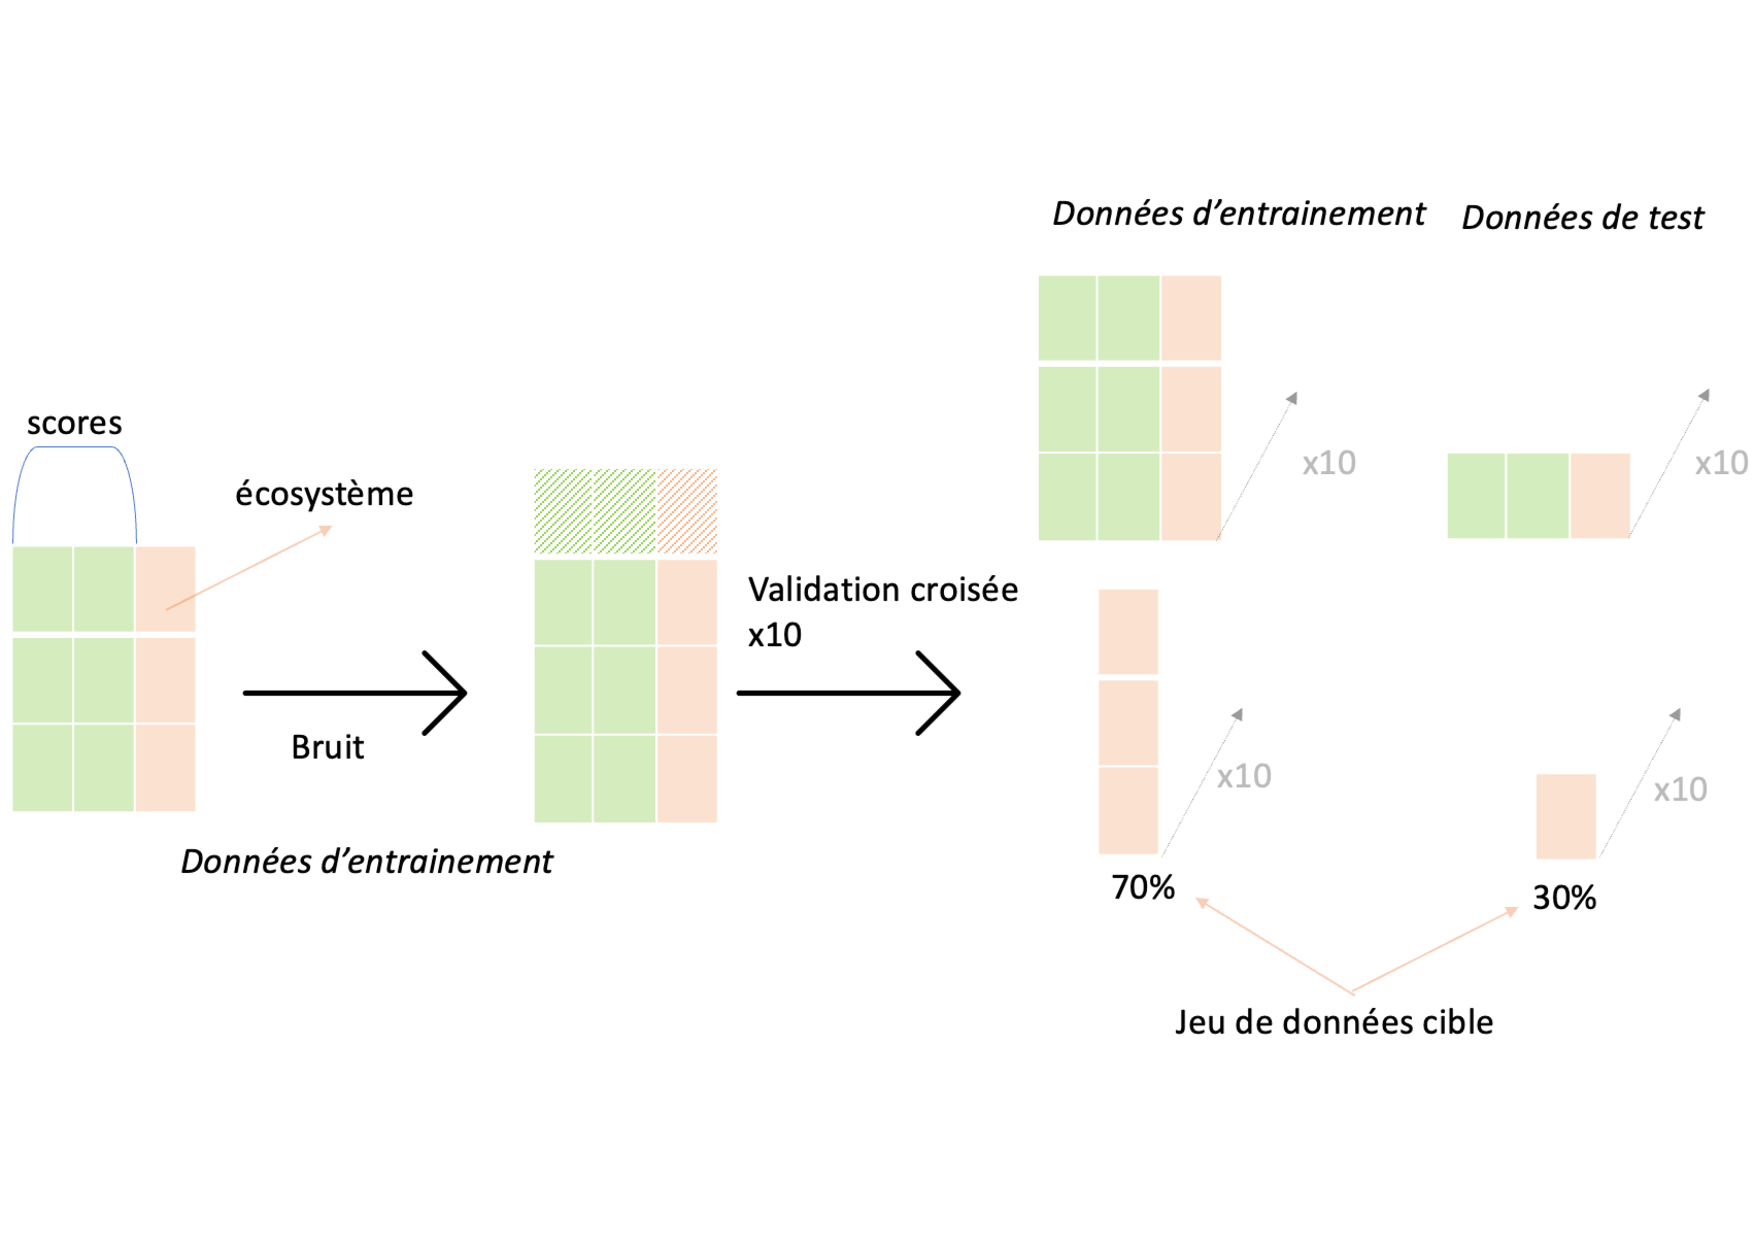
\includegraphics[width=\textwidth]{img/cocomico/svm.pdf}
    \caption{\textbf{Preparation des données afin d'être utilisé par le SVM.} Le jeu de données d'entrainement est constitué du ou des scores d'interaction (en vert) et de l'écosystème associé à ces scores (saumon). Le jeu de donnée cible est consitué de l'écosystème que l'on souhaite prédire.}
    \label{fig:svm}
\end{figure}


En entrée, deux jeux de données sont fournis: un comportant l'écosystème que l'on souhaite prédire (jeu de donnée cible) et le second le ou les scores d'interaction avec leur écosystème (données d'entrainement). Nous avons bruité les données d'entrainement puis effectué 10 validations croisées sur les deux jeux de données. Cela consiste à partitionner aléatoirement 10 fois les jeux de donnée d'entrainement et cibles de la façon suivante: 70\% des jeux de données servent à entrainer le modèle et 30\% servent à le tester. Par exemple, si nous voulons prédire l'écosystème de la feuille à partir du score de coopération, seul le score de coopération sera pris en compte pour l'ensemble des écosystèmes dans les données d'entrainement, et seul l'écosystème de la feuille sera présent dans jeu de donnée cible. 

\paragraph*{Comparaison avec des outils numériques sur des données expérimentales}
Notre approche permet l'analyse de communauté de grande taille, et à ma connaissance, il n'existe pas de méthode qualitative permettant d'évaluer le potentiel de coopération et de compétition à l'échelle de la communauté. Nous avons donc comparé notre approche avec des méthodes numériques de référence basées sur des contraintes: SMETANA \citep{Zelezniak2015} et MiCOM \citep{diener2020}.

Ces deux outils ont été décrit dans le chapitre \ref{ch:edla}. Brièvement, SMETANA propose deux scores pour calculer la coopération  (MIP) et la compétition (MRO) dans une communauté. SMETANA calcule ses scores indépendamment du milieu de culture fourni en entrée et reflète les limites théoriques des interactions \citep{Machado2021}. Nous avons donc lancé SMETANA version 1.2.0 sur 250 communautés composées de 3 à 30 réseaux métaboliques reconstruits avec CarveMe \citep{Machado2018} sur une collection de génomes bactériens de référence du NCBI RefSeq (release 84)\footnote{\url{https://github.com/cdanielmachado/embl\_gems}}. Puis les scores de coopération (MIP) et de compétition (MRO) calculés par SMETANA sont comparés à ceux obtenu avec notre méthode. 

MICOM est originalement développé pour la modélisation du microbiote humain dans lequel des taux de croissances et des flux d'échanges métaboliques sont prédits. Nous avons utilisé MICOM version 0.32.0 sur 188 communautés issues d'une analyse métagénomique, de taille variant de 16 à 98 espèces \citep{diener2020}. Les modèles métaboliques proviennent de la base de données VMH \citep{Noronha.2018} et une curation a été faite sur les réactions de transports. En effet, afin de s'assurer que seules les graines du milieu nutritionnel sont utilisées comme substrat nutritif, nous avons retiré ces réactions des GEMs.  Enfin, nous avons lancé les simulations sur le milieu de culture donné par MICOM: \textit{vmh\_high\_fiber\_agora.qza}. Cependant, MICOM ne donne pas d'indice direct de coopération et de compétition. En utilisant la fonction \texttt{knockout\_taxa} nous avons mesuré l'impact de la perte d'un taxon sur la croissance d'un autre taxon. D'après la documentation de MICOM, une augmentation (resp. une diminution) du taux de croissance après l'étape de knockout indique une coopération (resp. compétition) entre ces deux espèces. En sommant les valeurs positives (resp. négatives), nous avons calculé un pseudo score de compétition (resp. coopération)  à l'échelle de la communauté. \\

Nous avons ensuite comparé les scores calculés par notre approche, ceux de SMETANA et MICOM sur des données réelles. Nous avons récupéré des génomes de souches bactériennes du kéfir \citep{Blasche.2021} et leurs réseaux métaboliques ont été reconstruit avec gapseq version 1.2 \citep{Zimmermann2021} et Pathway-Tools v.25.5 \citep{Karp2022} à l'aide de mpwt v.0.7 \citep{Belcour.2020}. Nous avons également comparé avec les modèles déjà reconstruits par l'outil CarveMe\footnote{\url{https://github.com/cdanielmachado/kefir\_paper}}. Ce jeu de données est composé de 2 communautés: une composée de 23 souches initialement cultivées sur milieu lait liquide et une de 31 souches initialement cultivées sur milieu lait solide; toutes deux contiennent les mêmes nutriments. En utilisant SMETANA, MICOM et notre approche nous avons calculé les potentiels de coopération et de compétition, ainsi que le nombre de métabolites échangeables.

\subsubsection{Implémentation}
Nous avons développé un paquet python nommé \ccmc, de l'anglais \textit{Cooperation and competition in microbial communities}. Le code source est disponible à l'adresse suivante : \url{https://gitlab.inria.fr/ccmc/CoCoMiCo} et est installable avec pypi \href{https://pypi.org/project/CoCoMiCo/}{https://pypi.org/project/CoCoMiCo/}.
Un tutoriel de notre approche a été montré dans un jupyter notebook \footnote{\url{https://gitlab.inria.fr/ccmc/CoCoMiCo/-/blob/dev-0-3/cocomico.ipynb?ref_type=heads}} dans lequel notre approche par raisonnement a été appliquée sur des communautés jouets décrites dans les Figures \ref{fig:concepts} et \ref{fig:scores}. Ce jupyter permet d'explorer les fonctionnalités intéressantes de notre approche, comme l'explicabilité de nos résultats. 

\section{Application et description de notre approche sur des communautés jouets}
Afin de garantir la bonne compréhension de la méthode, nous avons illustré par la Figure \ref{fig:concepts}, les concepts que nous avons décrits. \ccmc permet d'identifier les potentiels de coopération et de compétition au moyen d'un modèle basé sur le raisonnement. Pour y parvenir, l'ensemble des réseaux métaboliques de la communauté ainsi un descriptif du milieu nutritionnel (correspondant aux graines) ont été fourni, afin d'identifier les voies métaboliques activées. La Figure \ref{fig:concepts}a illustre les dépendances nécessaires ainsi que le fonctionnement de \ccmc. Toutes les notions métaboliques que sont: graines, produits, réactants, taxon, communauté et environnement ainsi que les relations entre elles sont montrées dans la sous figure \ref{fig:concepts}b. \\


\begin{figure}[H]
    \centering
    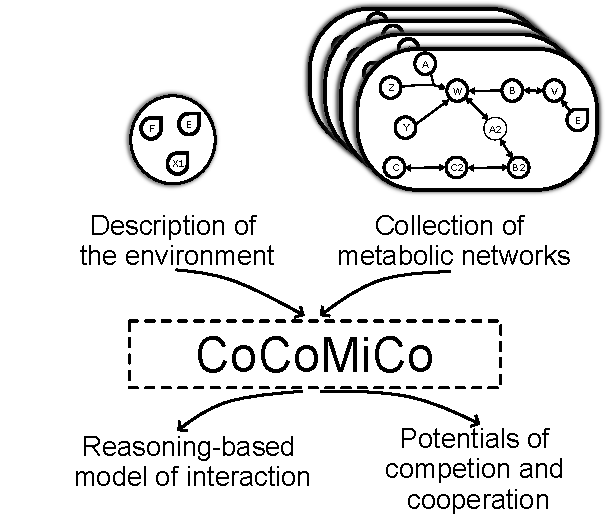
\includegraphics[width=\textwidth]{img/cocomico/concept.pdf}
    \caption{\textbf{Modèle basé sur le raisonnement et son application sur des données jouets.}
     (\textbf{a.}) L'approche générale de \ccmc est décrite. En entrée de l'outil, nous avons besoin d'une collection de GEMs décrivant les organismes présents dans la communauté, ainsi que l'ensemble des graines décrivant le milieu nutritionnel. En sortie, nous obtenons le vocabulaire contrôlé issu des règles logiques nous permettant de calculer les scores de coopération et de compétition.
(\textbf{b.}) Description de la base de faits générée par l'approche par raisonnement et appliquée à cette communauté jouet de 4 GEMs.}
    \label{fig:concepts}
\end{figure}

Pour s'exempter de toute confusion avec un algorithme utilisant seulement la topologie des graphes métaboliques pour l'identification de métabolites d'intérêt, \textit{i.e.} échangeable et limitant, le Figures \ref{fig:mono-polyopsonie} et \ref{fig:scores}a,b représentent la modélisation faite au moyen de l'algorithme d'expansion d'Ebenhoh \citep{Ebenhoh2004}. À partir d'un ensemble de graines, que sont X1, F et E, le \texttt{scope} métabolique de chaque espèce, \textit{i.e.} l'ensemble de composés productibles, est indiqué en jaune dans les Figure \ref{fig:scores}a et b, montrant par la même occasion, les réactions activées par l'intermédiaire des échanges (en bleu) \citep{Frioux2018}. 

\begin{figure}[H]
    \centering
    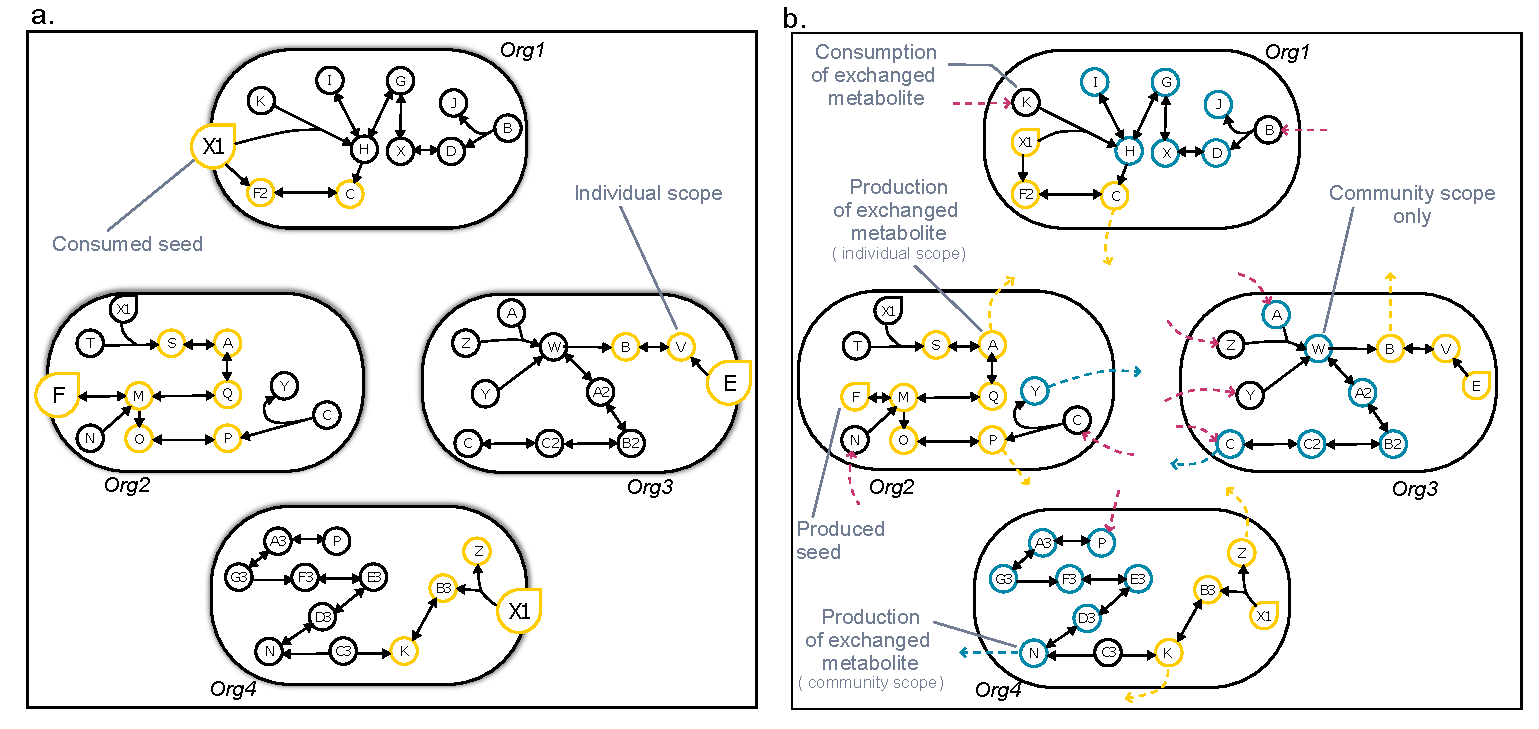
\includegraphics[width=\textwidth]{img/cocomico/score.pdf}
    \caption{  (\textbf{a.}) Potentiel métabolique de chaque GEM de la communauté. Les métabolites en jaune sont les nouveaux métabolites productibles à partir des graines X1, E et F. (\textbf{b.}) Illustration du potentiel métabolique de la communauté. Le potentiel individuel pour chaque GEM est représenté en jaune et le potentiel métabolique de la communauté en bleu, montrant ainsi la plus-value de la communauté. Les flèches sortantes en bleues (resp. jaune) montrent les métabolites échangeables lorsque les GEMs sont en communauté (individuel). Les flèches roses montrent la consommation des métabolites échangés.
    }
    \label{fig:scores}
\end{figure}

Pour cette communauté de taille 4, le \texttt{scope} métabolique de chaque taxon, représenté par le listing \ref{lst:individual-scope}, est donc composé de:

\begin{lstlisting}[mathescape=True,label={lst:individual-scope}, caption={Résultat du scope de chaque taxon},captionpos=b]
Org4: {X1, Z, B3, K}
Org3: {E, V, B}
Org2: {F, M, O, P, Q, A, S}
Org1: {X1, F2, C}
\end{lstlisting}

En communauté, représenté par la sous figure \ref{fig:scores}b, le \texttt{scope} communautaire est composé alors de:
\begin{lstlisting}[mathescape=True,label={lst:individual-scope}, caption={Résultat du scope communautaire},captionpos=b]
% scope metabolique communautaire
Org4: {N, D3, E3, F3, G3, A3, P}
Org3: {C, C2, B2, A2, W, A}
Org2: {Y}
Org1: {J, D, X, G, H, I}
\end{lstlisting}

Le base de connaissance que nous avons décrie nous permet de toujours identifier le taxon associé à la production du métabolite. A l'échelle de la communauté, le \textit{scope} communautaire, montre la plus-value métabolique de la communauté. Pour inférer les scores de coopération et de compétition, \ccmc met en avant les métabolites polyopsonistes, \textit{i.e.} les composés échangés et les graines qui sont co-consommés, et les métabolites monopsonistes, \textit{i.e.} ceux qui sont consommé uniquement que par un organisme. Ces deux concepts sont illustrés dans la Figure \ref{fig:mono-polyopsonie}.

\begin{figure}[H]
    \centering
    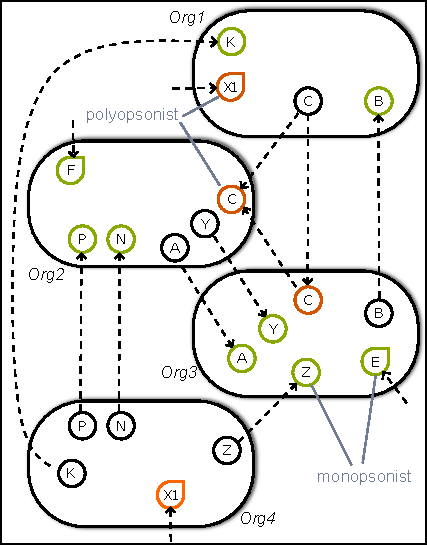
\includegraphics[width=0.6\textwidth]{img/cocomico/poly-monoopsonie.pdf}
    \caption{\textbf{Modèle basé sur le raisonnement et son application sur des données jouets.}
    Résumé des graines prédites comme consommées et des métabolites échangeables. Les éléments considérés comme polyopsonistes sont en orange, où le nombre de GEMs les consommant est strictement supérieur à 1. Ceux en vert traduisent la monoopsonie, un seul GEM les consomme. Pour chaque cas, \ccmc nous informe sur le producteur et le consommateur de chaque métabolite.}
    \label{fig:mono-polyopsonie}
\end{figure}

Ainsi, les métabolites polyopsonistes et monopsonistes sont:
\begin{lstlisting}[mathescape=True,label={lst:individual-scope}, caption={Métabolites considérés comme limitants (polyopsonie) et ceux non limitants (monopsonie)},captionpos=b]
% polyopsonie
X1: {Org1, Org4}
C: {Org2, Org3}

%monopsonie
Org3: {Z, A, Y, E}
Org2: {F, P, N}
Org1: {K}
\end{lstlisting}

En comparaison avec les travaux précédents se basant sur la même approche de raisonnement \citep{Frioux2018}, \ccmc décrit systématiquement les échanges métaboliques ainsi que les substrats limitants afin d'inférer des potentiels de coopération et de compétition à l'échelle de la communauté, que sont respectivement $CooP$ et $ComP$. En plus de cette inférence, deux autres métriques que sont $\delta$ et $\rho$ sont calculées montrant respectivement la plus-value des échanges métaboliques sur le nombre de composés productibles et le nombre de réactions activées grâce aux échanges. \\

Les figures \ref{fig:scores2},\ref{fig:scores3} et \ref{fig:scores4} montrent à travers des exemples, repris en partie des Figures \ref{fig:mono-polyopsonie} \ et  \ref{fig:scores}, les valeurs prises par $CooP$, $ComP$, $\delta$ et $\rho$. À travers ces communautés jouets de différentes compositions taxonomiques et à partir d'un même milieu de culture (E,F et X1), l'évolution des scores face à des perturbations est montrée.  


Dans les sous figures \ref{fig:scores2}a et b, la plus-value de l'organisme 4 est illustrée par les scores calculés par \ccmc. Nous avons observé que seul les scores de coopération ne varient pas, car le nombre de métabolites polyopsonistes et le nombre d'échanges restent identique. Cependant, les deux métriques $\delta$ et $\rho$ informent mécanistiquement sur l'impact de l'organisme 4 par rapport à l'organisme 2. En effet, 5 fois plus de métabolites sont devenus productibles et 10 fois plus de réactions ont été nouvellement activées avec l'organisme 4. Des hypothèses de dépendances métaboliques peuvent être générées ainsi que sur la définition d'une communauté plus coopérative: seul le nombre de métabolites échangé doit-être pris en compte, le score de coopération, sa robustesse à des changements ou encore les plus-values de productions métaboliques.

\begin{figure}[H]
    \centering
    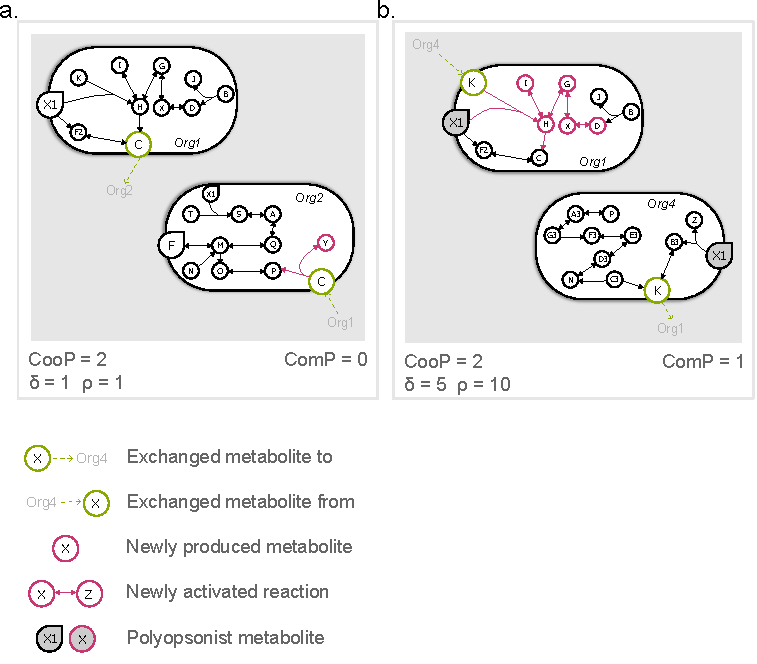
\includegraphics[width=\textwidth]{img/cocomico/score-taille-2.pdf}
    \caption{\textbf{Application de \ccmc sur les exemples jouets} (\textbf{a et b}). L'ensemble des concepts expliqués en amont sont représentés sur cette communauté de taille 2. Les scores de coopération et de compétition, respectivement \textit{CooP} et \textit{ComP}, ainsi que les plus-values métaboliques et réactionnelles, respectivement $\delta$ et $\rho$ sont également représentées. Les composés en verts sont les composés échangésn rose les composés produits grâce aux échanges}
    \label{fig:scores2}
\end{figure}


Dans la Figure \ref{fig:scores3}, la plus-value de l'organisme 4 est également montré dans une communauté de taille 3, dans laquelle, les organismes 1 et 2 sont présents dans les deux cas. Le nombre de substrats polyopsonistes étant identique (2), le score de compétition ne bouge pas, cependant la communauté de la sous figure \ref{fig:scores3}b semble moins coopérative (score de coopération passant de 9 à 8) alors que le nombre de composés échangés reste le même dans les deux cas: 4. Les sous métriques $\rho$ et $\delta$ sont sensiblement identiques. Nous pouvons noter que ces deux communautés de taille 3 semblent moins compétitives que les communautés de taille 2 de la Figure \ref{fig:scores2}, malgré le nombre d'échanges plus important. 

\begin{figure}[H]
    \centering
    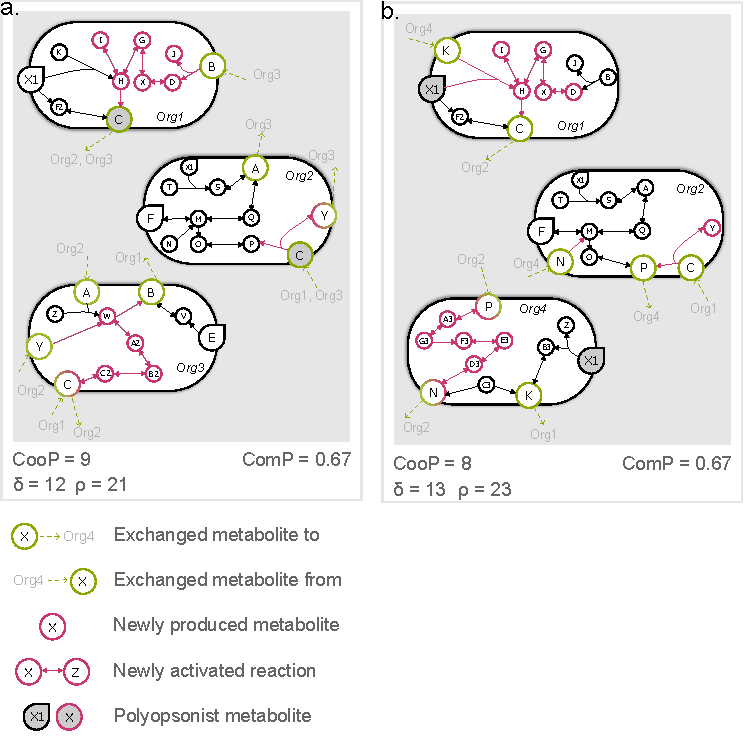
\includegraphics[width=\textwidth]{img/cocomico/score-taille-3.pdf}
    \caption{\textbf{Application de \ccmc sur les exemples jouets} (\textbf{a et b}). L'ensemble des concepts expliqués en amont sont représentés sur cette communauté de taille 3. Les scores de coopération et de compétition, respectivement \textit{CooP} et \textit{ComP}, ainsi que les plus-values métaboliques et réactionnelles, respectivement $\delta$ et $\rho$ sont également représentées.  Les composés en verts sont les composés échangésn rose les composés produits grâce aux échanges}
    \label{fig:scores3}
\end{figure}


Enfin, la Figure \ref{fig:scores4} montre les scores finaux obtenus pour la communauté que nous avons décrits dans les Figures \ref{fig:scores} et \ref{fig:mono-polyopsonie}. Nous pouvons identifier que les organismes 3 et 4 doublent le score de coopération (\textit{cooP} = 17) sans rentrer en compétition (\textit{comP = 1}). 

\begin{figure}[H]
    \centering
    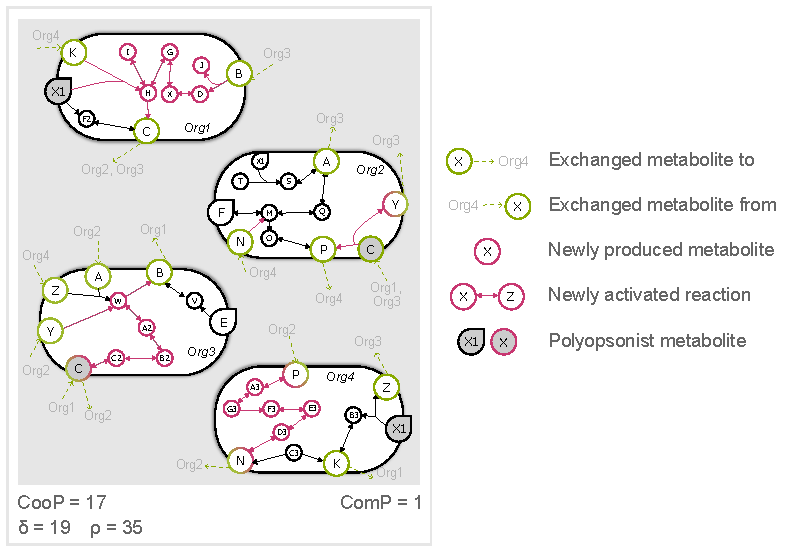
\includegraphics[width=\textwidth]{img/cocomico/score-taille-4.pdf}
    \caption{\textbf{Application de \ccmc sur un exemple jouet} L'ensemble des concepts expliqués en amont sont représentés sur cette communauté de taille 4. Les scores de coopération et de compétition, respectivement \textit{CooP} et \textit{ComP}, ainsi que les plus-values métaboliques et réactionnelles, respectivement $\delta$ et $\rho$ sont également représentées.  Les composés en verts sont les composés échangésn rose les composés produits grâce aux échanges}
    \label{fig:scores4}
\end{figure}


\section{Application de notre approche par raisonnement sur des communautés synthétiques}
Nous venons de décrire le fonctionnement de \ccmc sur des exemples jouets. Des informations plus complètes sont disponibles dans le jupyter notebook écrit à cet effet. \footnote{\url{https://gitlab.inria.fr/ccmc/CoCoMiCo/-/blob/dev-0-3/cocomico.ipynb?ref_type=heads}}

%Un 5ème factice, dénommé mixte, composé des 4 autres écosystèmes.

\subsection{Description des potentiels de coopération et de compétition à travers différents écosystèmes}
Afin de tester nos scores, nous avons appliqué \ccmc sur 50 communautés de taille différentes pour 4 écosystèmes: l'intestin, la feuille, la racine, et le sol.  Pour rappel, nous avons également lancé avec 2 milieux de culture différents: un générique et un spécifique de l'écosystème. Dans les paragraphes suivants, nous étudierons le comportement de nos scores de compétition et de coopération dans les 4 écosystèmes.

\subsubsection*{Application de \ccmc à partir d'un milieu de culture générique}
Une première analyse avec un milieu nutritionnel générique est faite afin de comparer les résultats entre eux, puis une seconde avec un milieu nutritionnel propre à chaque écosystème sera présentée, afin d'identifier l'impact d'un changement de milieu sur les scores d'interaction. \\

Lorsque l'on créé un modèle par raisonnement se basant sur la topologie d'un objet, ici le réseau métabolique, nous devons vérifier si les résultats que l'on obtient ne sont pas directement reliés à cette topologie. Pour cela, nous avons vérifié qu’il n’existe pas de corrélation entre la similarité des réseaux métaboliques et les potentiels de coopération et de compétition.

\paragraph*{Similarité des réseaux métaboliques et potentiels d'interaction}
Notre approche par le raisonnement est une méthode d'inférence qualitative ne permettant pas de calculer flux métaboliques, et se repose donc sur la topologie du modèle métabolique. Nous avons testé la similarité des réseaux en terme de composition en réactions métaboliques calculée par l'indice de Jaccard (voir méthodes) avec les potentiels de coopération et de compétition pour chaque écosystème. La figure \ref{fig:similarite} et la Table \ref{tab:corjacpot} montrent qu'il n'y a pas corrélation entre la topologie des réseaux métaboliques et les potentiels d'interaction obtenus. Ainsi, l'utilisation d'un formalisme discret prenant en compte les conditions environnementales apporte des plus d'informations que la seule structure des réseaux pour analyser et caractériser des communautés bactériennes.

\begin{figure}[H]
    \centering
    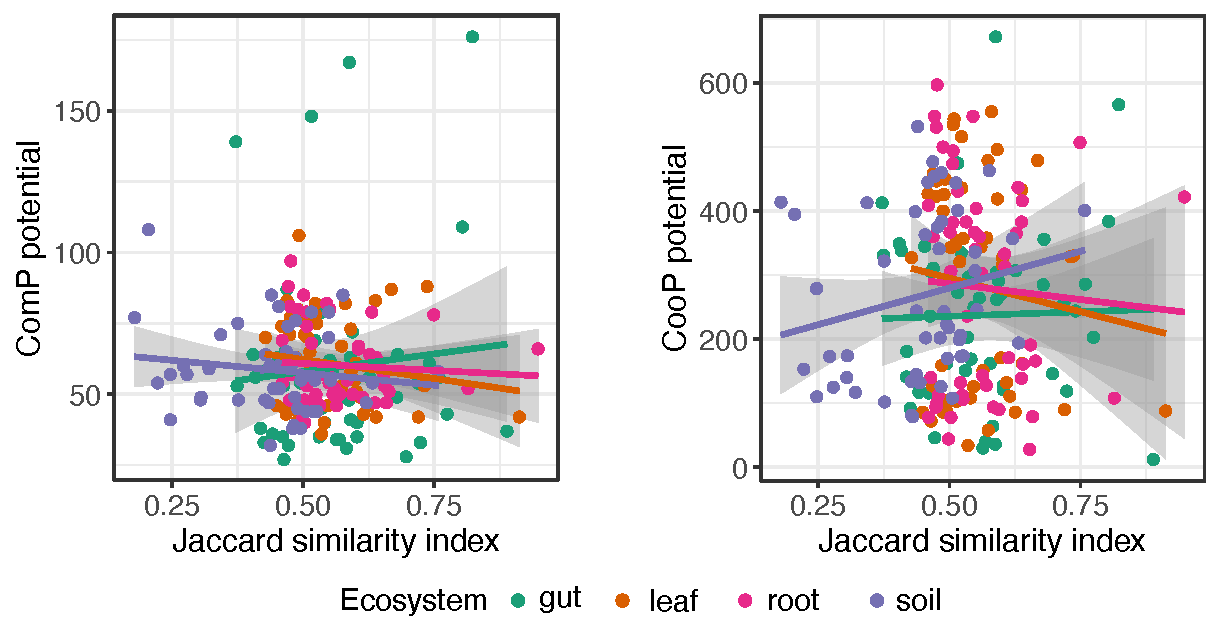
\includegraphics[width=\textwidth]{img/cocomico/similarite.pdf}
    \caption{Scores de coopération et de compétition calculé pour 50 communautés de taille 2 de chaque écosystème. Pour chaque paire, la similarité des réseaux métaboliques a été calculée par l'indice de Jaccard.  Les tests statistiques sont montrés dans la Table \ref{tab:corjacpot}}
    \label{fig:similarite}
\end{figure}

\begin{table*}[h!]
\resizebox{\linewidth}{!}{%
\begin{tabular}{llllllll}
\toprule
          &    & \multicolumn{3}{l}{Competition}    & \multicolumn{3}{l}{Cooperation}    \\ 
ecosystem & n & S        & rho estimate & p. value & S        & rho estimate & p. value \\ 
\midrule
gut       & 50 & 21889.05 &-0.051       & 0.724   & 21128.12 & -0.014      & 0.920 \\
leaf      & 50 & 21483.21 &-0.031       & 0.827    & 23141.56 & -0.111      & 0.441 \\
root      & 50 & 22515.28& -0.081      &0.575    & 23113.31 & -0.109     & 0.447 \\
soil      & 50 & 15744.51 &0.243       & 0.087    & 22505.37 & -0.080      & 0.577 \\
\bottomrule
\end{tabular}%
}
\caption{Résultat des tests de corrélation (Spearman) entre l'indice de similarité de Jaccard et les scores de potentiels d'interaction}
\label{tab:corjacpot}
\end{table*}


\paragraph*{Description globale des potentiels}
Les scores de coopération et de compétition calculés pour chaque écosystème (intestin, sol, racine et feuille) sont représentés par la Figure \ref{fig:ecosystem}. La sous figure \ref{fig:ecosystem}a illustré que les scores varient à la fois selon l'écosystème et à la fois selon la taille de la communauté. En effet, la taille de la communauté est fortement corrélée aux scores d'interaction calculés par \ccmc : (\textsf{ComP}: Spearman $\rho = 0.74$, $P < \num{2.2e-16}$, 
\textsf{CooP}: Spearman $\rho = 0.80$, $P < \num{2.2e-16}$). La forte association avec la coopération n'est pas surprenante, puisque le nombre de voies métaboliques augmente avec l'ajout de nouveaux membres dans la communauté, ainsi que le nombre de métabolites échangeables. Comme la compétition se repose en partie sur le nombre de métabolites échangés, l'augmentation du potentiel de compétition lorsque que la taille de la communauté augmente est attendue. 

Nous avons ensuite testé si, indépendamment de la taille de la communauté, les potentiels de coopération et de compétition de chaque écosystème étaient discernables. Les résultats, illustrés par la sous figure \ref{fig:ecosystem}b, montrent que la compétition semble avoir plus de difficulté à différencier les communautés de la feuille, de la racine et du sol entre eux. Au contraire, le potentiel de coopération, différencie bien la racine et la feuille du sol mais peine à différencier la racine de la feuille.

\begin{figure}[H]
    \centering
    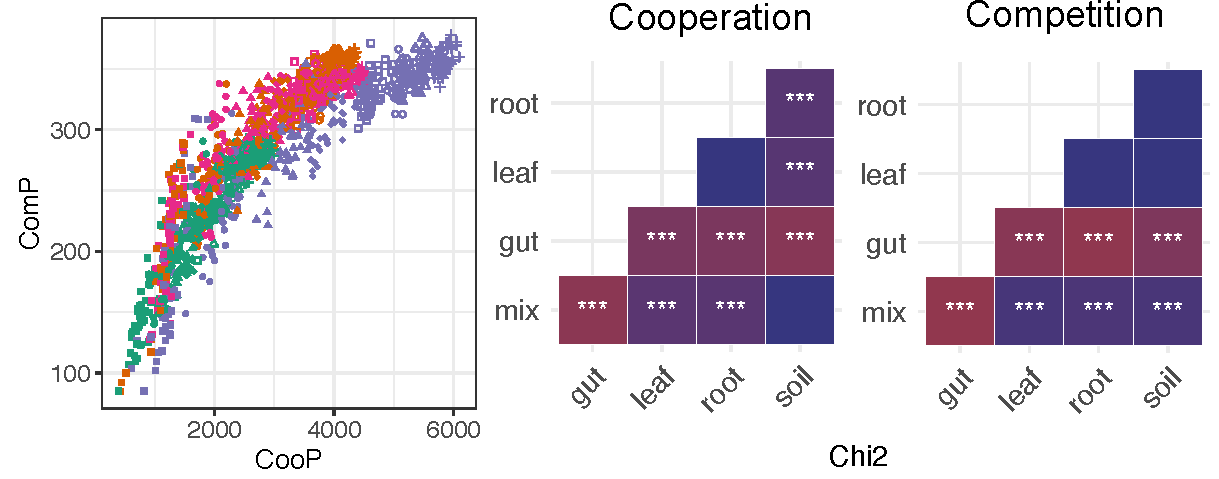
\includegraphics[width=\textwidth]{img/cocomico/coop-comp-ecosys.pdf}
    \caption{(a) Distribution des scores de coopération et de compétition dans des communautés simulées de 5 à 150 bactéries isolées de l'intestin, de la racine, de la feuille et du sol. (b) Résultats d'un test du $\text{chi}^2$ de Kruskal-Wallis comparant les potentiels de coopération et de compétition obtenu en (a) entre écosystème.  (*)  $P$-values ajustées (Benjamini-Hochberg): $P < 0.05$,
    (**) $P$-values ajustées (Benjamini-Hochberg): $P < 0.01$,
    (***) $P$-values ajustées(Benjamini-Hochberg): $P < 0.001$. La communauté \textit{mixte} est un mélange composé équitablement des écosystèmes de la racine, de la feuille, du sol et de l'intestin. }
    \label{fig:ecosystem}
\end{figure}

on observe que, les communautés de l'intestin présentent des scores de compétition et de coopération moins élevé que les autres écosystèmes. Cette observation est explicable par le nombre de métabolites échangés comme indiqué dans Table \ref{table:coop-comp-ecosys} dans laquelle le sol a en moyenne deux fois plus d'échangés que dans les communautés de l'intestin. Nous avons également remarqué que les nombres de métabolites échangés pour la feuille et la racine sont proches. Nous avons supposé que ces résultats pussent être reliés à la diversité taxonomique des GEMs utilisés dans la création des communautés synthétiques (voir Figure \ref{supp:taxo}). Ainsi, au regard de la Figure \ref{supp:taxo}, les communautés du sol et de l'intestin, possédant les plus grandes diversités taxonomiques, ont montré les plus grandes et les plus petites valeurs de compétitions respectivement, suggérant que la diversité taxonomique ne semble pas être le seul facteur déterminant les potentiels d'interaction. En revanche, la similitude des scores d'interaction pour les écosystèmes de la feuille et de la racine, semble être corrélée avec leur diversité taxonomique proche.
%
%
%\begin{table}[H]
%\centering
%\begin{adjustbox}{width=1\textwidth}
%\begin{tabular}{|c|c|c|c|c|c|}
%\hline
% & sol & intestin & racine & feuille & mixte \\
%\hline
%métabolites échangeables & $1024\pm 18$ & $588\pm 33$ & $678\pm 18$ &$693\pm 10$ & $1211\pm 31$ \\
%CooP & $3943\pm 65$ & & & & $4663\pm 115$ \\
%ComP & $263\pm 5$ & & & & $330\pm 9$\\
%
% \hline
%\end{tabular}
%\end{adjustbox}
%\caption{\textbf{Moyenne des scores d'interactions ainsi que du nombre de métabolites échangeables pour tous les écosystèmes et pour une taille de communauté de 150.}}
%\label{table:coop-comp-ecosys}
%\end{table}


\begin{table}[H]
\centering
\begin{adjustbox}{width=1\textwidth}
\begin{tabular}{|c|c|c|c|c|c|}
\hline
 & sol & intestin & racine & feuille & mixte \\
\hline
métabolites échangeables & $\textbf{1516}\pm 27$ & $\textit{709}\pm 45$ & $1171\pm 64$ &$1105\pm 11$ & $\textbf{1525}\pm 53$ \\
CooP & $\textbf{5833}\pm 102$ & $\textit{2739} \pm 175$ & $4361 \pm 137$ & $4273 \pm 40$ & $\textbf{5877}\pm 189$ \\
ComP & $\textbf{355}\pm 9$ & $\textit{276} \pm 11$ & $345 \pm 3$ & $\textbf{357} \pm 4$ & $\textbf{384}\pm 12$\\

 \hline
\end{tabular}
\end{adjustbox}
\caption{\textbf{Moyenne des scores d'interactions ainsi que du nombre de métabolites échangeables pour tous les écosystèmes et pour une taille de communauté de 150.}}
\label{table:coop-comp-ecosys}
\end{table}

Afin de vérifier statistiquement nos observations, nous avons comparé les scores de compétition et de coopération pour chaque taille et par écosystème (voir Figure \ref{fig:diff-potentials})

\begin{figure}[H]
    \centering
    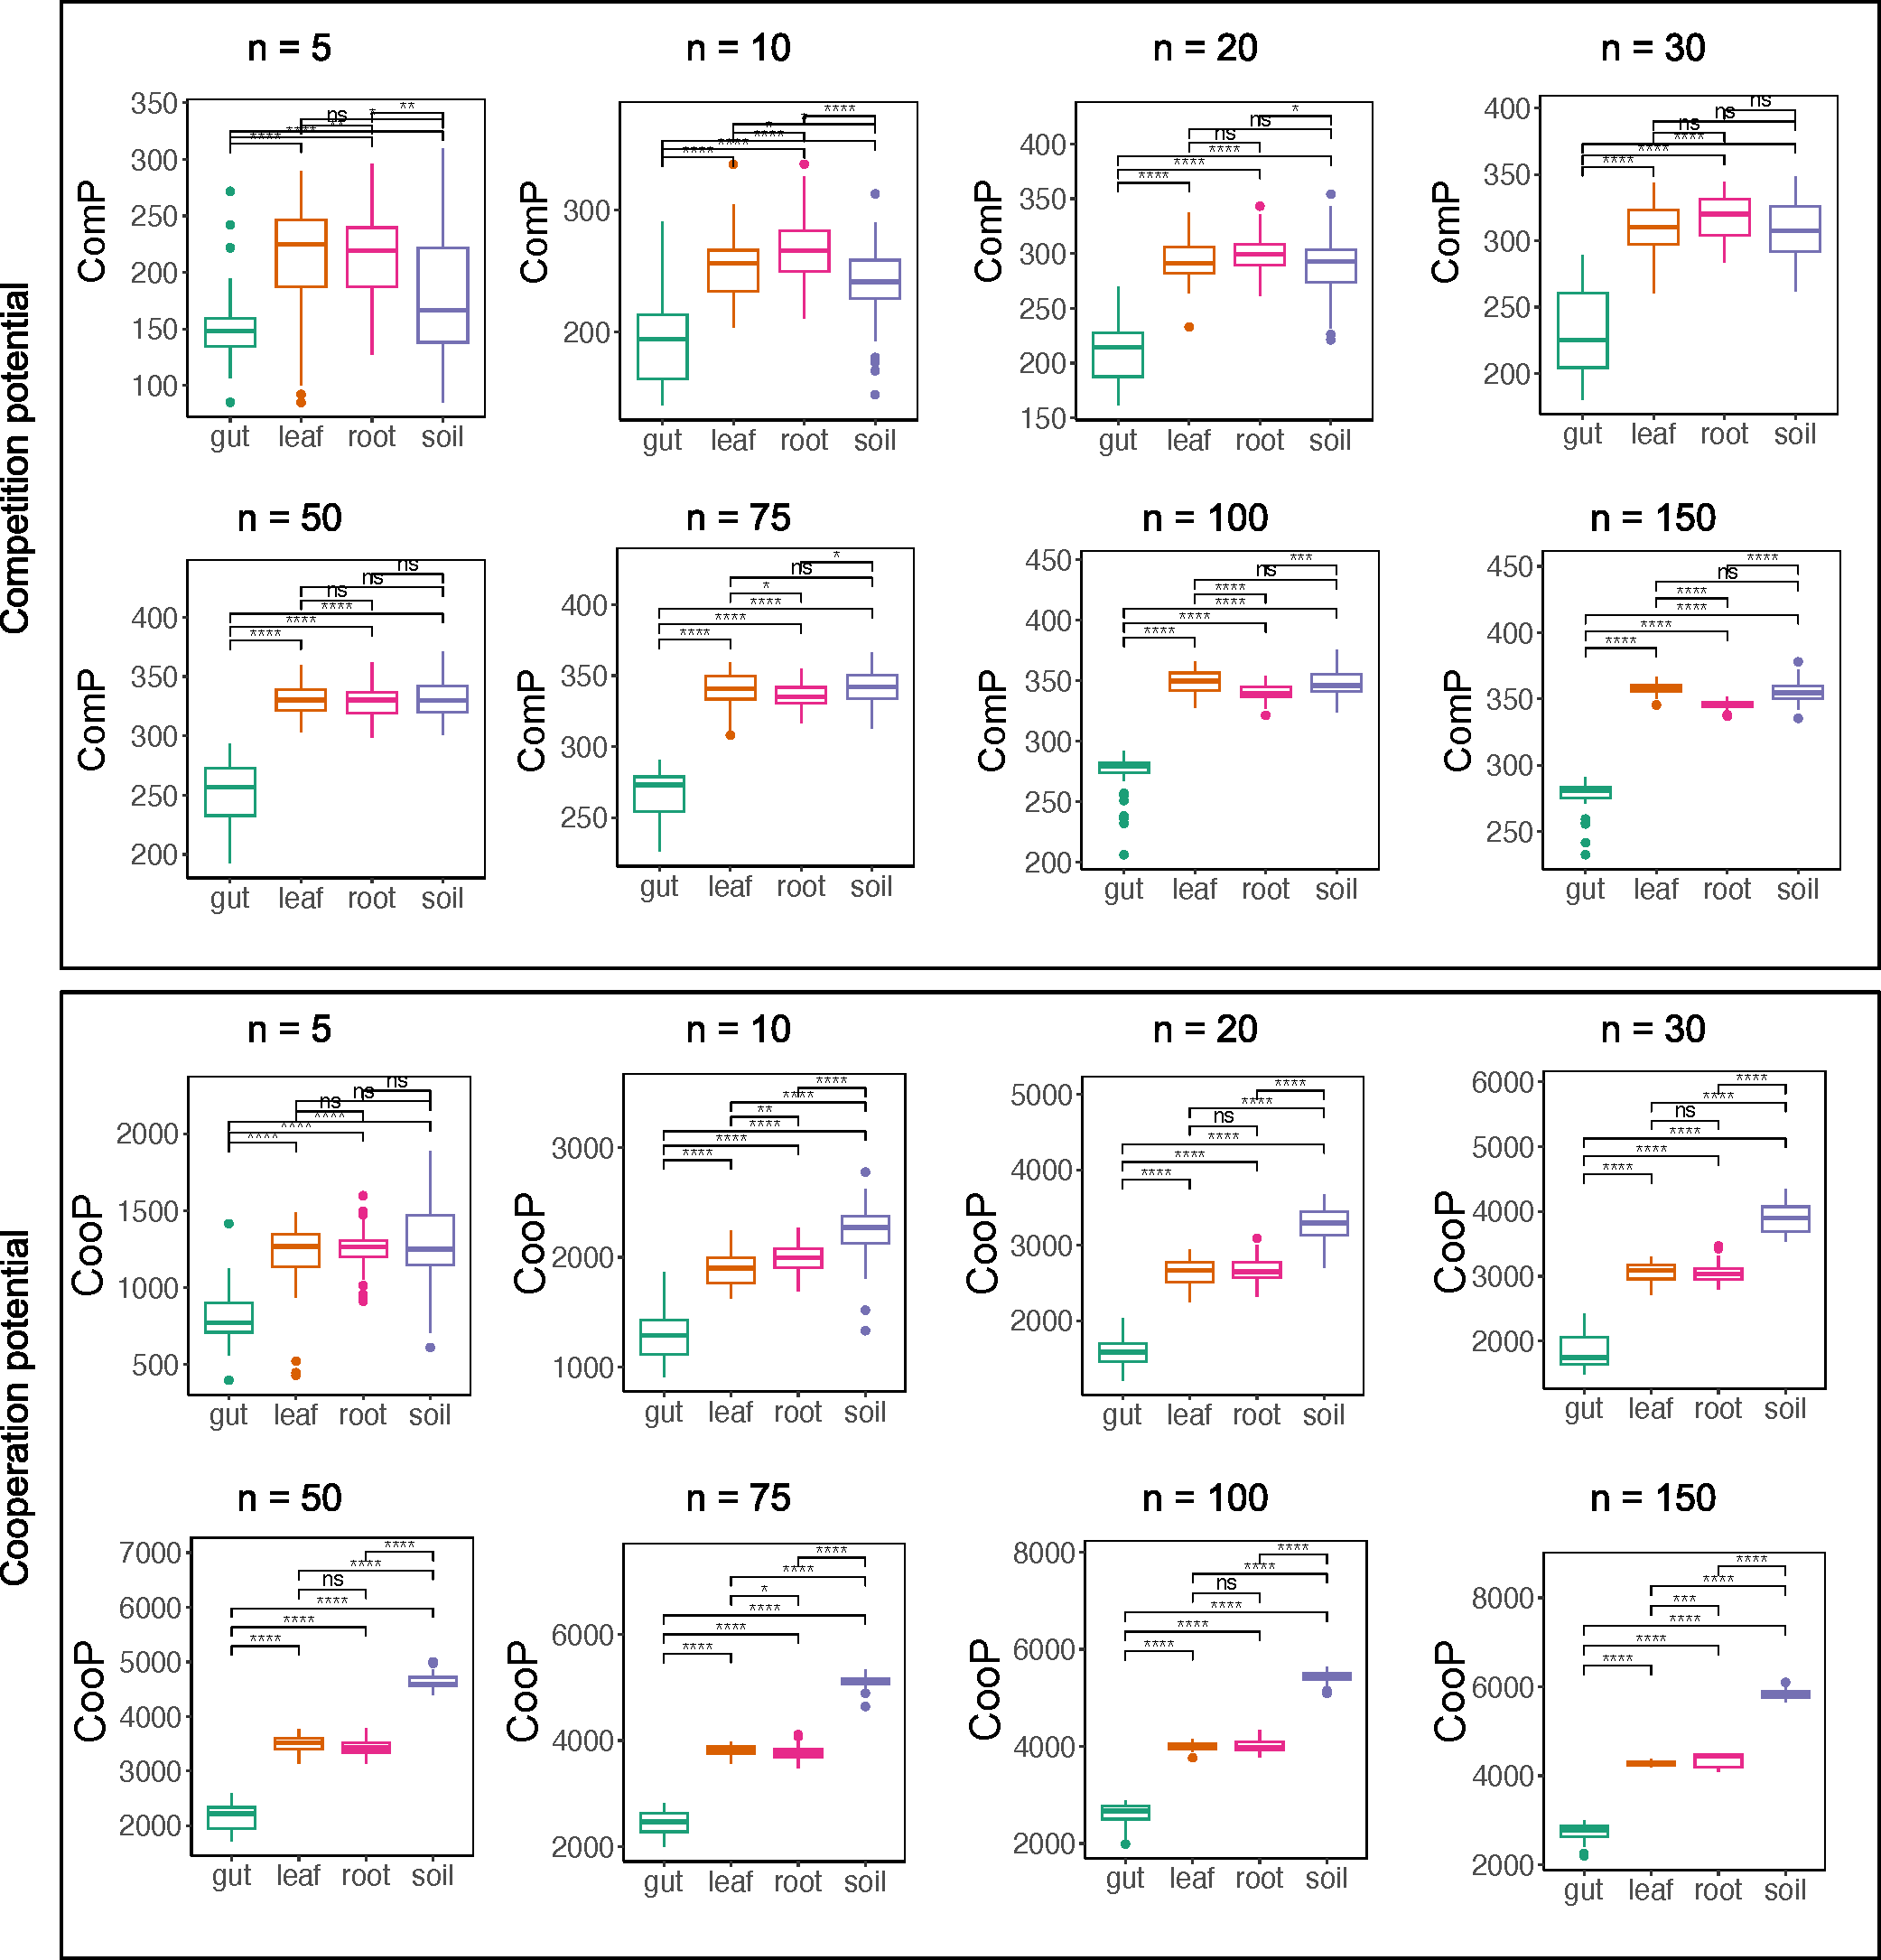
\includegraphics[width=\textwidth]{img/cocomico/ecosysteme_diff_potentials.pdf}
    \caption{Distribution des scores de coopération et de compétition dans des communautés simulées de 5 à 150 bactéries isolées de l'intestin, de la racine, de la feuille et du sol. Une comparaison de moyenne avec le test de Wilcoxon a été faite. (*)  $P$-values ajustées (Benjamini-Hochberg): $P < 0.05$,
    (**) $P$-values ajustées (Benjamini-Hochberg): $P < 0.01$,
    (***) $P$-values ajustées(Benjamini-Hochberg): $P < 0.001$.}
    \label{fig:diff-potentials}
\end{figure}

Nous montrons que la compétition distingue globalement moins bien les communautés de petites tailles (entre 5 et 30), surtout entre les écosystèmes de la racine, de la feuille et du sol, ce qui est cohérent avec les observations décrites plus haut. Le score de coopération semble être plus apte à discerner des communautés > 10 taxa, sauf entre les écosystèmes de la feuille et de la racine. Les communautés de grandes tailles étant plus réalistes, ces dernières sont distinguées par nos potentiels d'interactions, apportant de la confiance à nos métriques. \\

Un point nouveau, et peu documenté dans la littérature était la mesure de l'impact d'une modification de la composition bactérienne sur les scores de coopération et de compétition. Notre approche ne pouvant prendre en compte des abondances, nous avons modélisé l'impact d'un changement discret en ajoutant ou en enlevant une nouvelle espèce dans chacune des communautés de tailles 3 à 150 de l'intestin (voir Figure \ref{fig:added-value}). Par rapport à la communauté originale, les scores de coopération et de compétition ne permettent plus de distinguer la plus-value d'ajouter ou de retirer une espèce à partir d'une communauté de taille 10. Cela suggère donc que l'effet d'une modification d'un facteur biotique peut-être capturé par \ccmc uniquement pour des écosystèmes de petites tailles. Les communautés de tailles réelles ne verront pas leurs potentiels d'interactions changés significativement.


\begin{figure}[H]
    \centering
    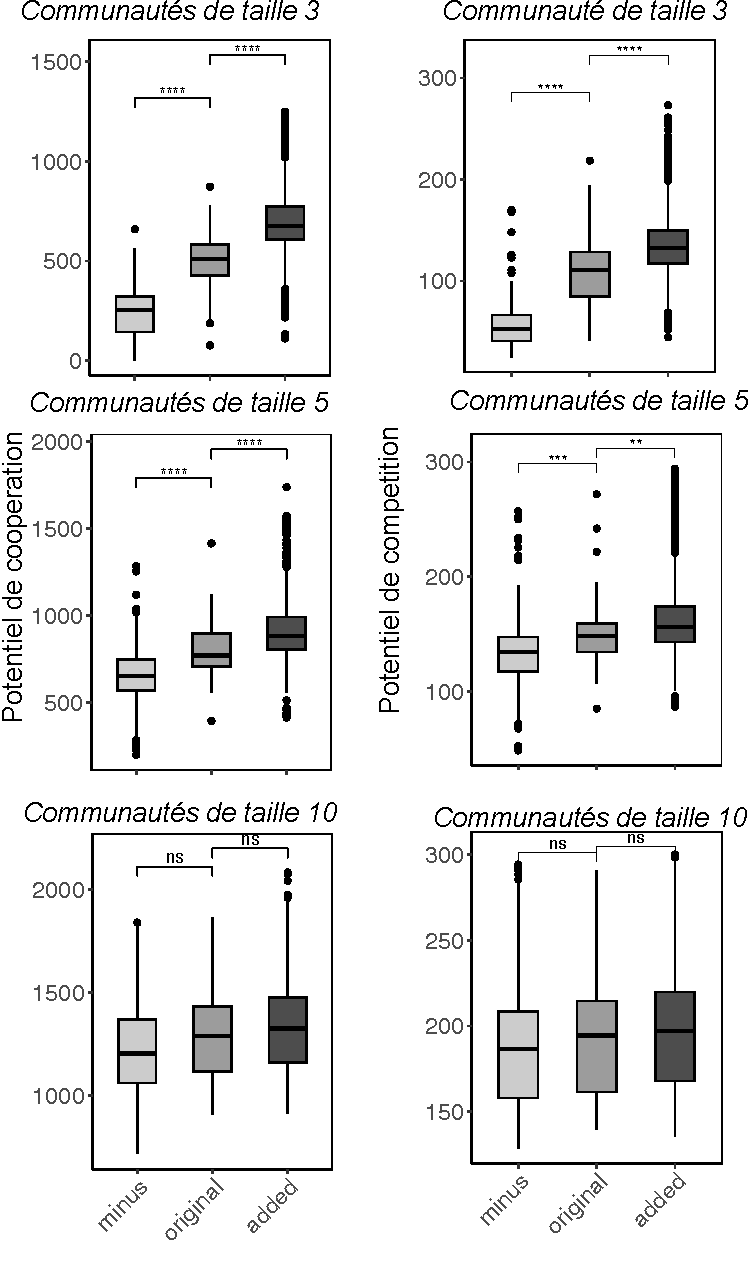
\includegraphics[width=0.8\textwidth]{img/cocomico/added-value.pdf}
    \caption{Effet d'ajouter ("added") ou de retirer une espèce ("minus") sur les potentiels de coopération et de compétition pour chaque communauté. Le test de comparaison de moyenne Wilcoxon a été utilisé sur des communauté de taille 3 à 10 sur l'écosystème de l'intestin.}
    \label{fig:added-value}
\end{figure}

\paragraph*{Comparaison des potentiels d'interaction propres aux écosystèmes avec ceux d'un écosystème factice}

Nous avons en plus créé une $5^{\grave{e}me}$ communauté artificielle composée d'une combinaison des réseaux métaboliques appartenant aux 4 autres écosystèmes, dénotée "mixte". Cette communauté non réaliste permet de vérifier que les potentiels de coopération et de compétition sont spécifiques aux écosystèmes, et permettrait donc de discerner des communautés non plausibles. Nous avons remarqué que le potentiel de compétition a permis de distinguer l'écosystème mixte des autres, ce qui n'est pas le cas pour le score de coopération où le sol et un écosystème factice serait similaire du point de vue de ce potentiel d'interaction (voir Figures \ref{fig:ecosystem} et \ref{fig:diff-potentials}). Nous retrouvons également ce résultat dans la Table \ref{table:coop-comp-ecosys} où les valeurs de coopération, de compétition et du nombre de métabolites échangés sont particulièrement proche de l'écosystème du sol.  Lorsque l'on compare par taille de communauté (voir Figure \ref{fig:mix-diff-potentials}) les deux potentiels de coopération et de compétition arrivent à différencier l'écosystème factice. En revanche, comme illustré dans la Figure \ref{fig:ecosystem}, l'écosystème du sol et le mixte semblent être identique de point de vue de la coopération.

\begin{figure}[H]
    \centering
    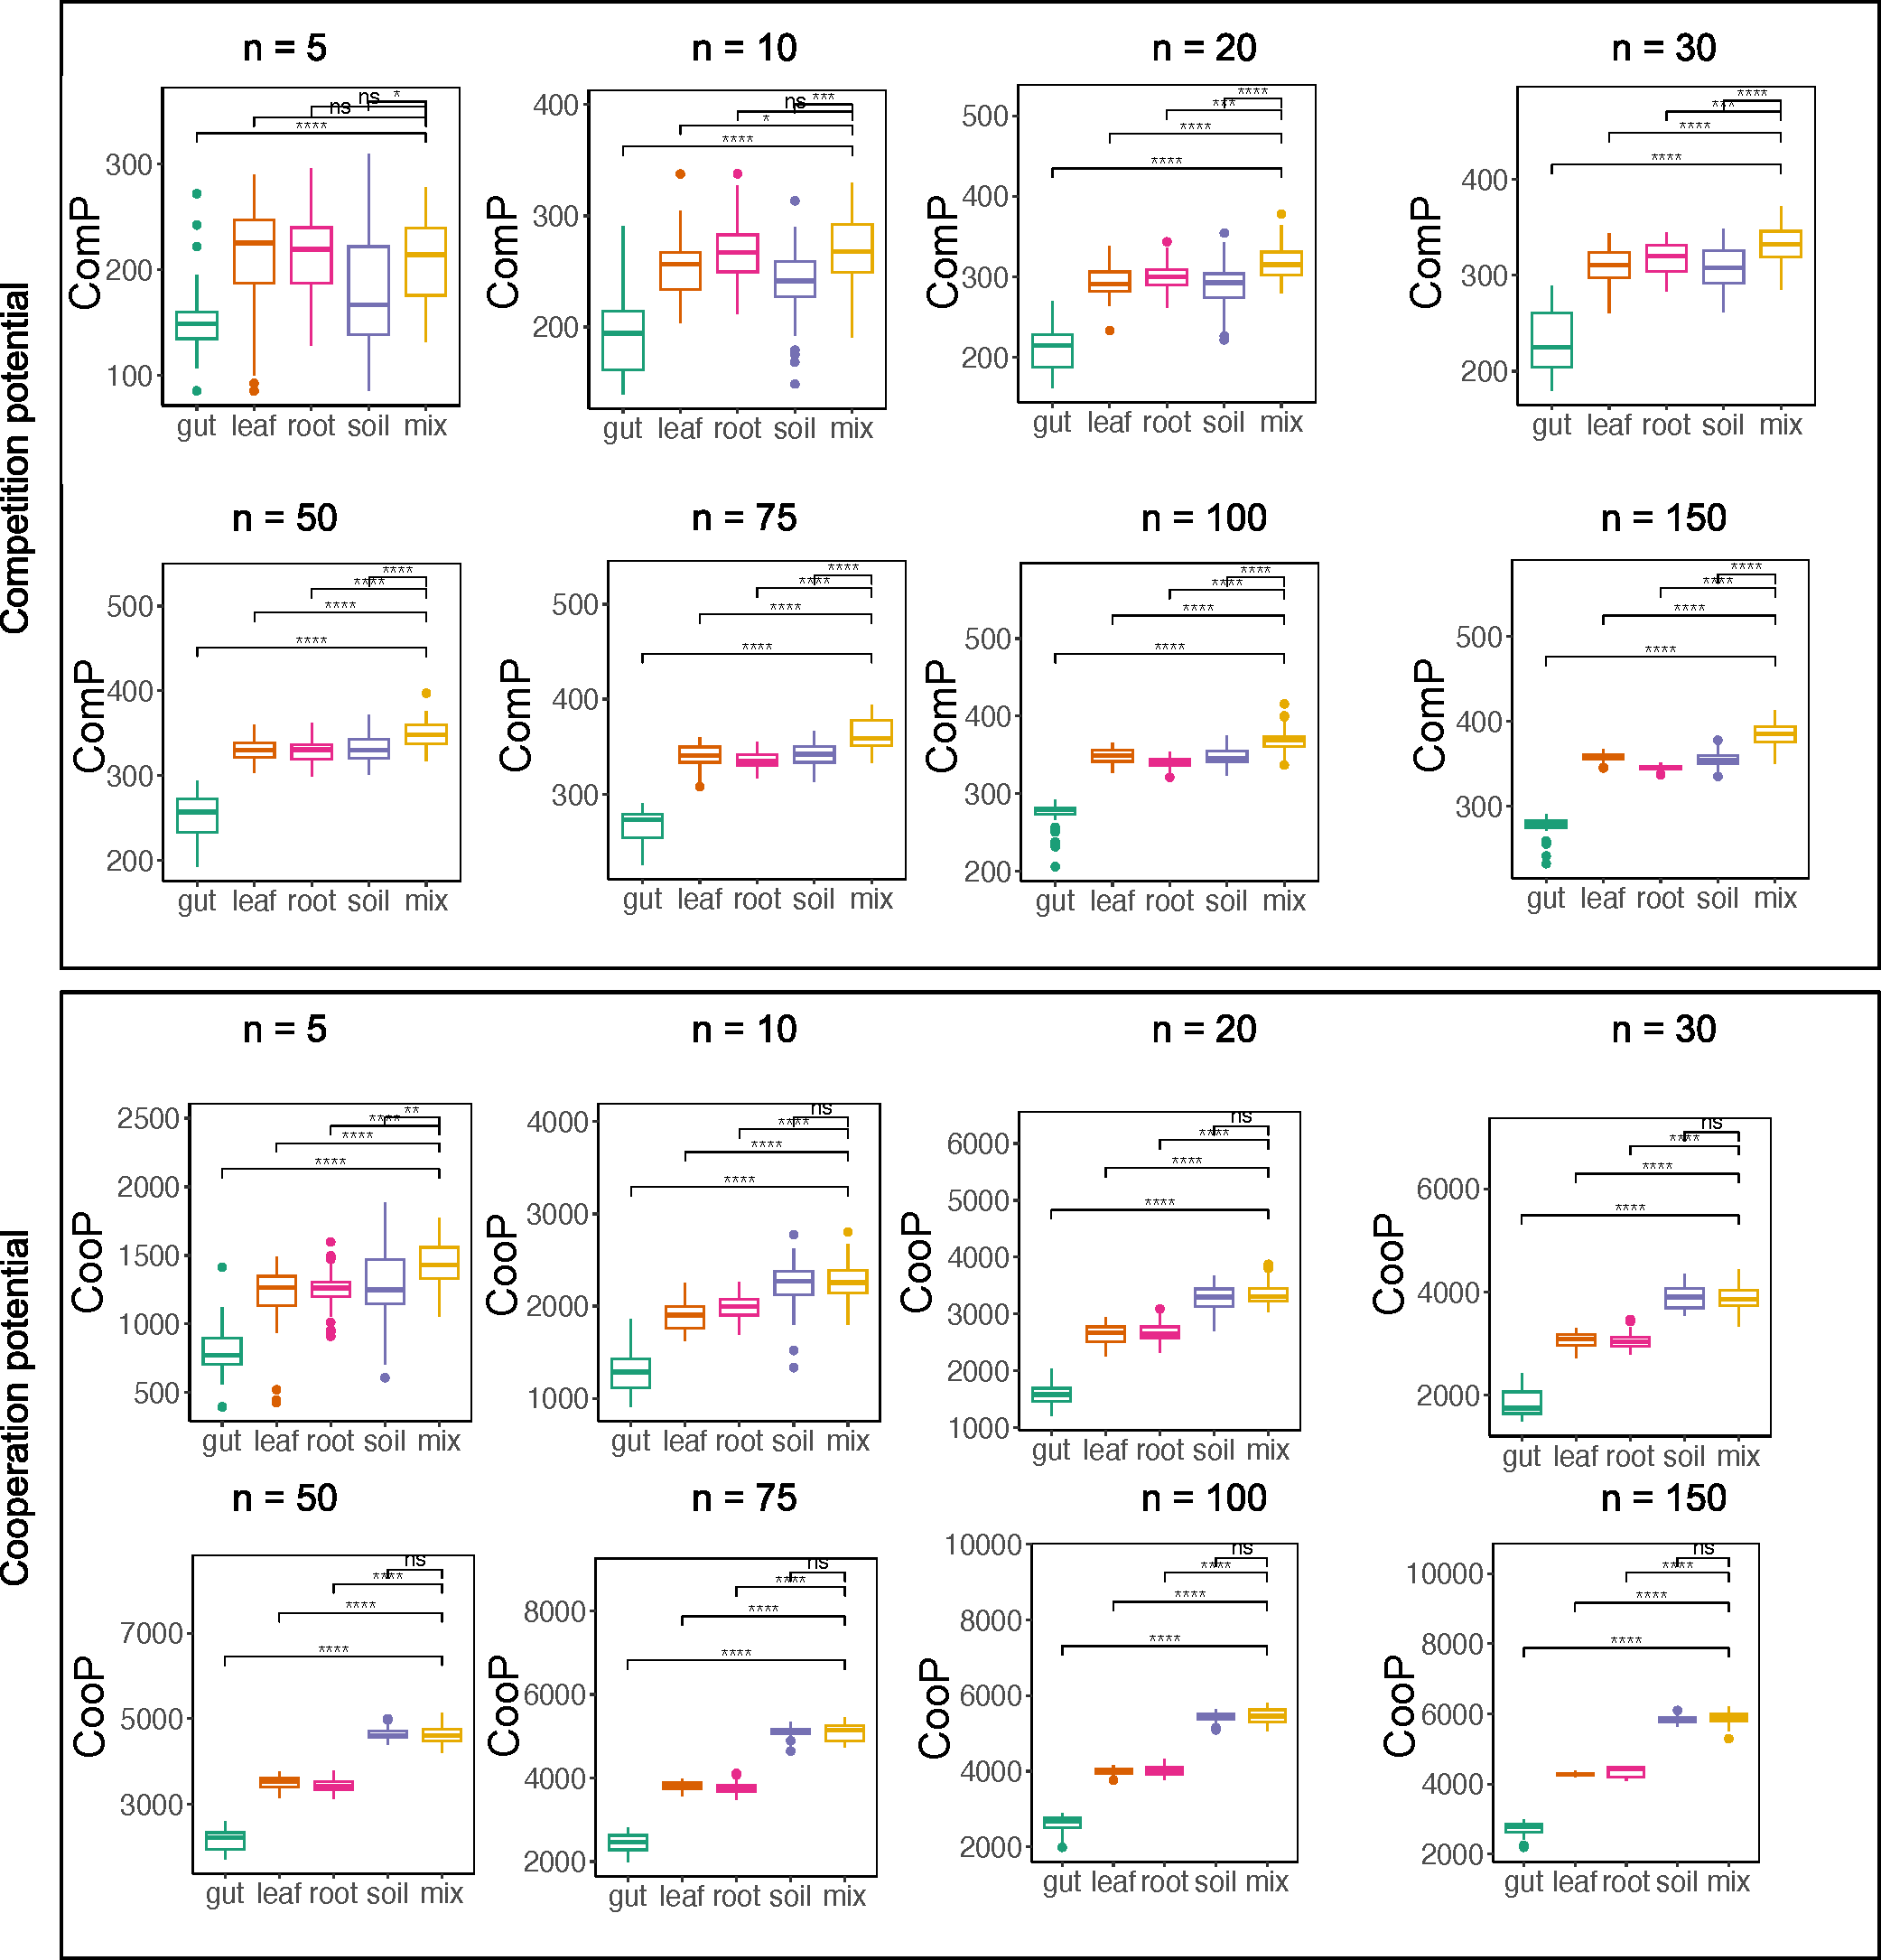
\includegraphics[width=\textwidth]{img/cocomico/mix_ecosystem_diff_potentials.pdf}
    \caption{Distribution des scores de coopération et de compétition dans des communautés simulées de 5 à 150 bactéries isolées de l'intestin, de la racine, de la feuille, sol et du mixte. Seule une comparaison deux à deux avec le mixte a été faite. La comparaison de moyenne est faite avec le test de Wilcoxon. (*)  $P$-values ajustées (Benjamini-Hochberg): $P < 0.05$,
    (**) $P$-values ajustées (Benjamini-Hochberg): $P < 0.01$,
    (***) $P$-values ajustées(Benjamini-Hochberg): $P < 0.001$}
    \label{fig:mix-diff-potentials}
\end{figure}



Une étape terminale d'exploitation des potentiels d'interaction serait de pouvoir prédire des écosystèmes à partir d'un score de coopération et de compétition. Les résultats de ce test sont présentés dans le paragraphe suivant.

\paragraph*{Prédiction d'écosystème à partir de potentiel d'interaction}
Nous avons vu et démontré que les potentiels d'interaction semblent être en général spécifiques à des écosystèmes. Une hypothèse sous-jacente consiste à se demander si, à partir des potentiels d'interaction de coopération et de compétition de chaque écosystème, il est possible de prédire l'écosystème correspondant. Afin de tester et vérifier cette hypothèse, nous avons utilisé un SVM ( de l'\textit{anglais}, Support Vector Machine) non linéaire (voir méthodes). Les résultats sont présentés par la Table \ref{table:SVM}.



\begin{table}[h!]
\centering
\begin{adjustbox}{width=1\textwidth}
\begin{tabular}{|c|c|c|c|c|}
\hline
 & sol & intestin & racine & feuille\\
\hline
CooP & $0.67\pm 0.34$ & $\textbf{0.74}\pm \textbf{0.32}$ & $0.48\pm 0.34$& $0.53\pm 0.35$ \\
ComP & $0.40\pm 0.31$ & $\textbf{0.93}\pm \textbf{0.12}$ &$0.44\pm 0.29$ & $0.42\pm 0.23$\\
ComP et CooP & $\textbf{0.71}\pm\textbf{ 0.29}$ & $\textbf{0.74}\pm \textbf{0.32}$ & $0.49\pm 0.35$&$0.5\pm 0.39$\\

 \hline
\end{tabular}
\end{adjustbox}
\caption{Résultat de prédiction des écosystèmes de la racine, de la feuille, du sol et de l'intestin, à partir les graines génériques. Les colonnes correspondent aux écosystèmes que l'on souhaite prédire à partir d'uniquement le score de coopération (CooP), d'uniquement le score de compétition (Comp) ou une combinaison des deux (ComP et CooP).}
\label{table:SVM}
\end{table}

Nous pouvons voir qu'à partir des graines génériques, seul l'intestin semble pouvoir être prédit correctement par les 3 combinaisons de scores. Le score de compétition semble plus se démarquer avec une moyenne de 0.93. Ce chiffre peut être intéprété comme un probabilité d'obtenir le bon résultat. Ainsi, un score de 0.93 signifie que nous avons 93\% de chance de prédire l'écosystème de l'intestin à partir du score de compétition. L'écosystème du sol semble être uniquement prédictible avec une combinaison du score de coopération et de compétition. En revanche, prédire les écosystèmes de la feuille et de la racine ne semble être faisable. Une hypothèse pouvant expliquer cette observation est la diversité taxonomique de ces deux écosystèmes qui n'est pas suffisamment distincte et génère des potentiels métaboliques proches, ayant pour conséquence des scores d'interaction similaires.


\subsubsection*{Application de \ccmc à partir d'un milieu de culture spécifique}
Nous avions utilisé un milieu de culture générique pour toutes les communautés pour comparer les potentiels d'interaction entre eux. Afin d'identifier une possible gamme des potentiels de coopération et de compétition propre à chaque écosystème, un milieu de culture spécifique de l'intestin et un milieu commun aux 3 autres écosystèmes ont été générés. 

\begin{figure}[H]
    \centering
    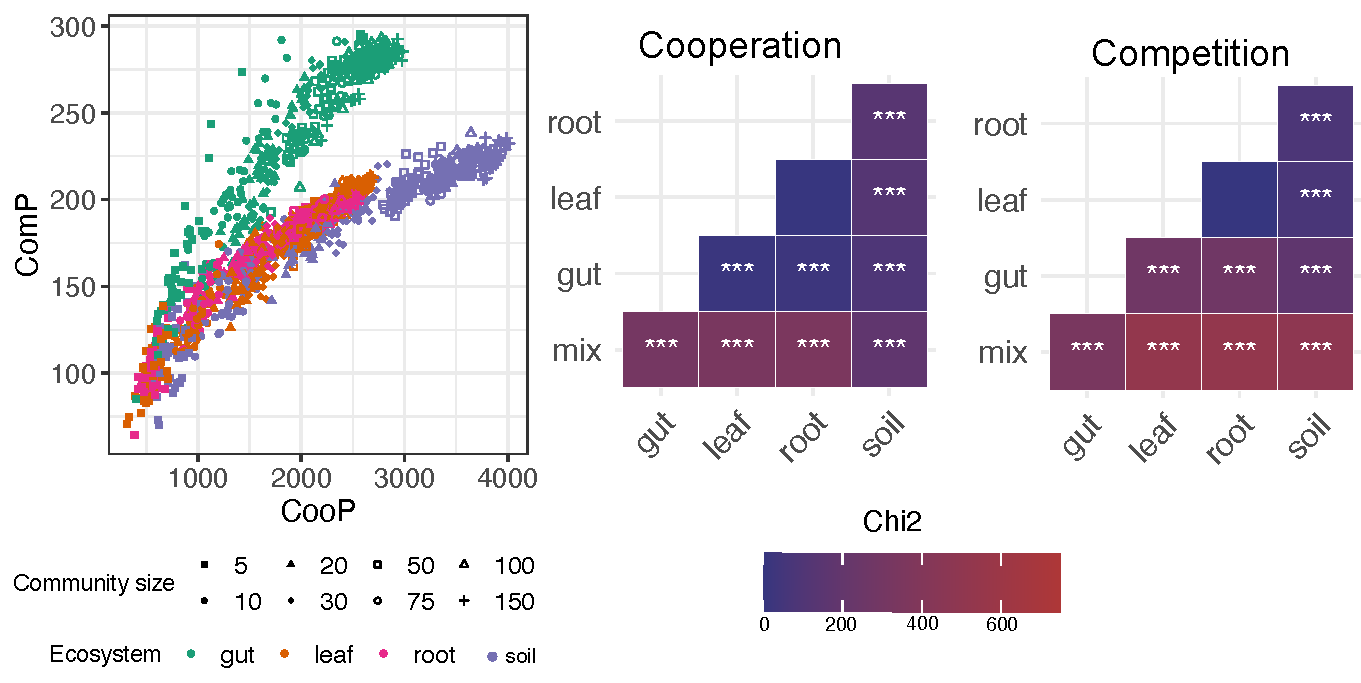
\includegraphics[width=\textwidth]{img/cocomico/coop-comp-ecosys-specific.pdf}
    \caption{(a) Distribution des scores de coopération et de compétition dans des communautés simulées de 5 à 150 bactéries isolées de l'intestin, de la racine, de la feuille et du sol. (b) Résultats d'un test du $\text{chi}^2$ de Kruskal-Wallis comparant les potentiels de coopération et de compétition obtenu en (a) avec ceux de la communauté mixte. }
    \label{fig:ecosystem-specific}
\end{figure}

Il existe des différences notables entre la Figure \ref{fig:ecosystem-specific}, utilisant environnement nutritionnel spécifique et la Figure \ref{fig:ecosystem}, utilisant un milieu générique. L'intestin semble avoir des scores de compétitions plus importants, et la valeur maximale de coopération est réduite à 4000 contre 6000 dans la Figure \ref{fig:ecosystem}. Lorsque l'on compare les potentiels de coopération et de compétition sans tenir compte de la taille de la communauté, les deux potentiels distinguent presque tous les écosystème. En effet, la racine et la feuille ne semble pas être significativement différent. Malgré cette amélioration, les potentiels d'interaction ne permettent toujours pas de prédire correctement des écosystèmes (voir Table \ref{table:SVM-specific})\\


\begin{table}[h!]
\centering
\begin{adjustbox}{width=1\textwidth}
\begin{tabular}{|c|c|c|c|c|}
\hline
 & sol & intestin & racine & feuille\\
\hline
CooP & $\textbf{0.90}\pm \textbf{0.15}$ & $0.48\pm0.23$ & $0.56\pm 0.37$& $0.47\pm 0.34$ \\
ComP & $0.66\pm 0.25$ & $\textbf{0.96}\pm \textbf{0.04}$ &$0.63\pm 0.39$ & $0.49\pm 0.33$\\
ComP et CooP & $\textbf{0.79}\pm\textbf{ 0.29}$ & $\textbf{0.87}\pm \textbf{0.15}$ & $0.59\pm 0.40$&$0.44\pm 0.35$\\

 \hline
\end{tabular}
\end{adjustbox}
\caption{Résultat de prédiction des écosystèmes de la racine, de la feuille, du sol et de l'intestin, à partir les graines spécifiques. Les colonnes correspondent aux écosystèmes que l'on souhaite prédire à partir d'uniquement le score de coopération (CooP), d'uniquement le score de compétition (Comp) ou une combinaison des deux (ComP et CooP). }
\label{table:SVM-specific}
\end{table}

Le résultat de la Table \ref{table:SVM-specific} indique qu’il n’est toujours pas possible de déterminer le potentiel d'interaction permettant de prédire un écosystème. Cependant, la combinaison des deux scores ainsi que l'utilisation de graines spécifique, semblent permettre la prédiction de l'intestin et du sol avec plus de confiance.

\subsection{Comparaison avec des méthodes basées sur des contraintes et application à des données expérimentales}


Les résultats précédents ont montré une application \textit{in silico} des potentiels d'interaction. Dans la suite de ce chapitre, nous allons présenter deux cas d'étude utilisant des données de communautés pour analyser leurs potentiels de coopération et de compétition. Dans le premier cas, nous avons calculé les potentiels d'interaction avec \ccmc sur 250 communautés créés artificiellement, de taille 3 à 30 et comparé avec les scores obtenus par SMETANA. Puis, sur un jeu de données de MICOM, nous avons calculé les potentiels de coopération et compétition avec \ccmc sur 188 communautés issues d'une analyse métagénomique, allant d'une taille 16 à 98 et comparé ces potentiels avec ceux calculés avec MICOM. Dans le second cas, nous avons comparé les résultats de coopération et de compétition obtenus par MICOM, SMETANA et \ccmc sur 2 communautés du kéfir provenant de \citep{Blasche.2021}.

\subsubsection*{Comparaison de méthodes numériques dans le calcul de score d'interaction}
Dans cette section, nous présenterons les résultats de la première étude de cas. L'objectif est vérifié, pour une même communauté, si nos scores sont corrélés avec ceux d'outils reconnus de la littérature.
La première remarque est que notre score de coopération semble être corrélé avec les scores des méthodes numériques avec une corrélation avec un $\rho = 0.8$ et une p-value de $2.2^{-16}$ pour SMETANA et $\rho = 0.69 $ avec une p-value de $2.2^{-16}$ pour MICOM (voir Figure \ref{fig:ccmc-micom-smetana}).

\begin{figure}[H]
    \centering
    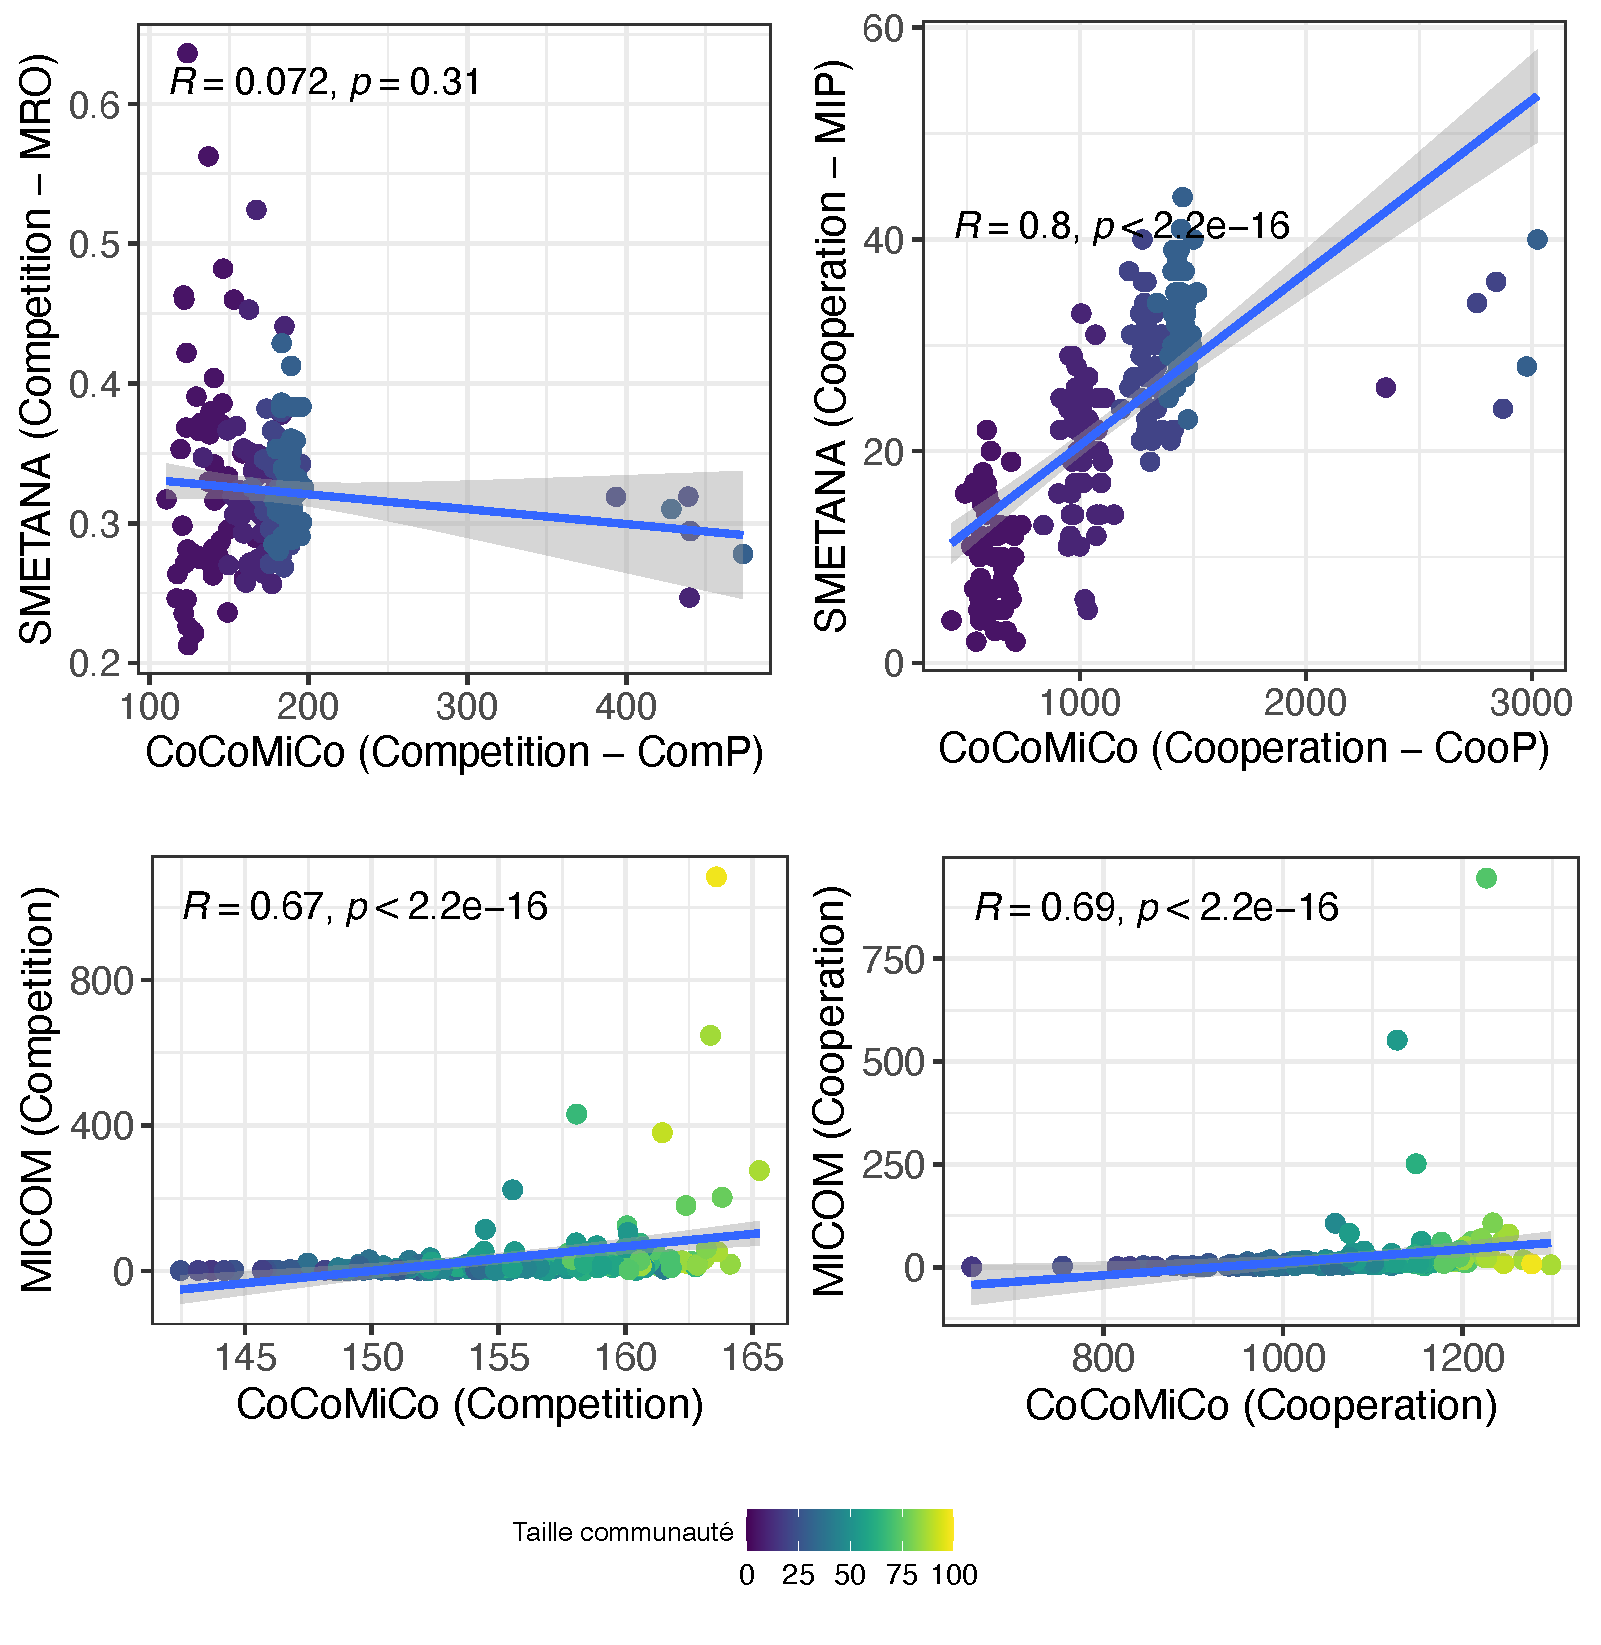
\includegraphics[width=\textwidth]{img/cocomico/ccmc-micom-smetana.pdf}
    \caption{\textbf{Comparaison des approches numériques MICOM et SMETANA avec notre approche}. (a) Comparaison des scores de coopération et de compétition développé par SMETANA,  respectivement MIP et MRO. 250 communautés de taille 3 à 30 ont été générées aléatoirement. (b) Comparaison des scores de coopération et de compétition \textit{ad hoc}  de MICOM sur 188 communautés issues d'analyses métagénomiques de taille 16 à 98 GEMs. En (a) et en (b), les corrélations ont été calculées avec la corrélation de Spearman.}
    \label{fig:ccmc-micom-smetana}
\end{figure}

La compétition en revanche, est seulement corrélée avec le score MICOM avec un $\rho$ de 0.67 et une p-value de $2.2^{-16}$. L'absence de corrélation avec le score SMETANA ($\rho$ de 0.072 avec une p-value de $0.31$) peut-être expliqué par la prise en compte d'un milieu de culture théorique minimum. Et donc, SMETANA ne prend pas en considération l'ensemble des éléments nutritifs comme dans \ccmc et MICOM. \\



Un point non négligeable à notifier est le temps de calcul des approches numériques. SMETANA ne pouvait être utilisé sur des communautés de taille supérieure à 30 pour une allocation mémoire de 10G. MICOM quant à lui, a permis l'analyse de grande communautés (98) mais met plusieurs heures pour une communauté avec 20G de mémoire. En comparaison, \ccmc a mis environ 3 minutes pour analyser une communauté de taille 150 avec 10G de mémoire.
De ce fait et malgré les différences méthodologiques, nous avons observé des similitudes et une rapidité d'exécution de \ccmc permettant la comparaison de potentiels de coopération et de compétition de communautés rapidement. De plus, les corrélations avec MICOM nous encouragent dans cette direction pour améliorer la précision des scores d'interaction.


\subsubsection*{Application sur des données expérimentales du kéfir}
Nous avons appliqué \ccmc ainsi que les deux approches numériques MICOM et SMETANA sur 2 communautés du kéfir de tailles différentes, 23 et 31. Lors de l'analyse des communautés sur milieu lait, les auteurs et autrices montrent un réseau d'interaction plus dense et globalement négatif pour la plus grande communauté, cultivé sur du gel d'agarose (noté lait-solide). L'ensemble des résultats est présenté dans la Table \ref{tab:kefirpotentials}. Tout d'abord, les réseaux métaboliques de Pathways-Tools étant dépourvus d'une fonction de biomasse nativement, l'application d'une méthode numérique était donc infaisable. 


\begin{table*}[h!]
\centering
\begin{adjustbox}{width=1\textwidth}
\begin{tabular}{cccccccc}
\toprule[1.3pt]
& \multicolumn{1}{c}{\multirow{2}{*}{Communauté}}   & \multicolumn{2}{c}{Pathway Tools}             & \multicolumn{2}{c}{CarveMe}                   & \multicolumn{2}{c}{gapseq}                                                                   \\
%\midrule[1.5pt]
        & & \multicolumn{1}{c}{Coopération} & Compétition & \multicolumn{1}{c}{Coopération} & Compétition & \multicolumn{1}{c}{Coopération} & Compétition                                               \\
\midrule[1pt]
\multicolumn{1}{c}{\multirow{2}{*}{CoCoMiCo}} & lait-liquide    & \multicolumn{1}{c}{{\begin{tabular}[c]{@{}l@{}} 1090.68 \\ (287) \end{tabular}}}           &     \multicolumn{1}{c}{123.26}         & \multicolumn{1}{c}{{\begin{tabular}[c]{@{}l@{}}2183.06 \\ (426) \end{tabular}}}     & {149.65}      & \multicolumn{1}{c}{{\begin{tabular}[c]{@{}l@{}}2039.34\\ (520) \end{tabular}}}            &     \multicolumn{1}{c}{233.74}         \\ \Cline{0.2pt}{2-8}
\multicolumn{1}{c}{} & lait-solide & \multicolumn{1}{c}{{\begin{tabular}[c]{@{}l@{}}1098.85\\ (278) \end{tabular}}}            &      \multicolumn{1}{c}{124.5}        & \multicolumn{1}{c}{{\begin{tabular}[c]{@{}l@{}}2651.19\\ (497) \end{tabular}}}     & {152.74}       & \multicolumn{1}{c}{{\begin{tabular}[c]{@{}l@{}}2039.39\\ (499) \end{tabular}}}            &      \multicolumn{1}{c}{243.53}                                 \\
\midrule[1pt]
\multicolumn{1}{c}{\multirow{2}{*}{SMETANA}} & lait-liquide    & \multicolumn{1}{c}{-}            &   \multicolumn{1}{c}{-}          & \multicolumn{1}{c}{{\begin{tabular}[c]{@{}l@{}}22\\ (59) \end{tabular}}}         & {0.329}       & \multicolumn{1}{c}{NA}            &      \multicolumn{1}{c}{{0.682}}    \\ \Cline{0.2pt}{2-8}
 \multicolumn{1}{c}{} & lait-solide & \multicolumn{1}{c}{-}            &   \multicolumn{1}{c}{-}          & \multicolumn{1}{c}{{\begin{tabular}[c]{@{}l@{}}22\\ (66) \end{tabular}}}           & {0.348}       & \multicolumn{1}{c}{NA}            &       \multicolumn{1}{c}{{0.693}}                               \\
\midrule[1pt]
\multicolumn{1}{c}{\multirow{2}{*}{MICOM}}  & lait-liquide    & \multicolumn{1}{c}{-}            &     \multicolumn{1}{c}{-}        & \multicolumn{1}{c}{{\begin{tabular}[c]{@{}l@{}}24.75\\ (99) \end{tabular}}}      & \multicolumn{1}{c}{{2.75}}        & \multicolumn{1}{c}{{\begin{tabular}[c]{@{}l@{}}22.435\\ (95) \end{tabular}}}           &       \multicolumn{1}{c}{{22.432}}      \\ \Cline{0.2pt}{2-8}
\multicolumn{1}{c}{} & lait-solide & \multicolumn{1}{c}{-}            &     \multicolumn{1}{c}{-}        & \multicolumn{1}{c}{{\begin{tabular}[c]{@{}l@{}}34.80\\ (109) \end{tabular}}}      & \multicolumn{1}{c}{{3.8}}         & \multicolumn{1}{c}{{\begin{tabular}[c]{@{}l@{}}31.476\\ (103) \end{tabular}}}            &        \multicolumn{1}{c}{{31.454}}                             \\
\bottomrule[1.3pt]
\end{tabular} 
\end{adjustbox}
\caption{\textbf{\ccmc,Smetana et MICOM sont appliqués sur les données expérimentales du kéfir \citep{Blasche.2021}} Les potentiels de coopération et de compétition sont obtenus pour les deux communautés cultivées sur lait liquide (n=23) ou lait solide (n=31) à partir des réseaux métaboliques reconstruits avec Pathway Tools, CarveMe et gapseq, et analysés MICOM, SMETANA et CoCoMiCo. Sans besoin d'une fonction objective, seul \ccmc a su déterminer les potentiels d'interaction sur les réseaux métaboliques issus de Pathway-Tool. SMETANA n'a pas pu déterminer le score de coopération signifiant qu'au moins une bactérie n'a pas pu pousser dans le modèle de communauté.
}
\label{tab:kefirpotentials}
\end{table*}


Globalement, les scores de potentiels de coopération et de compétition sont tous plus importants dans la plus grande communauté, facteur sûrement déterminé par la grande corrélation des scores avec la taille de la communauté (cf Figure \ref{fig:ecosystem}). Le nombre de métabolites échangés est moindre pour la plus petite communauté et pour les réseaux reconstruits avec Pathway-Tools et gapseq. Le réseau d'interaction positive 2 à 2 étant plus dense dans cette communauté, le nombre d'échanges métaboliques est attendu comme plus important. Les réseaux reconstruits avec CarveMe montrent l'inverse suggérant donc que la méthode de reconstruction peut impacter des propriétés intrinsèques à la communauté (ici, le nombre d'échanges).
Enfin, dernier point, notre méthode basée sur le raisonnement décrit un nombre de métabolites échangés nettement plus important que pour MICOM et SMETANA. Cela est également attendu puisque notre approche identifie toutes les interactions potentielles sans optimisation numérique. 

\section{Discussion et conclusion}
Dans ce chapitre nous avons proposé une méthode permettant d'analyser des communautés naturelles de façon rapide mettant en avant la coopération et la compétition. L'une des grandes forces de notre approche et son adaptabilité. En effet, l'obtention de réseaux métaboliques de bonnes qualité n'est pas courante dans l'analyse haut-débit de communautés microbiennes. Cette qualité vient d'une curation manuelle approfondie issue de la connaissance extraite de la littérature ou d'expériences \textit{in vitro}.  Ainsi, les réseaux métaboliques sont au stade d'ébauche et déterminer une réaction de biomasse peut être compliqué. Cependant, une approche comme \ccmc permet d'obtenir un aperçu des potentiels métaboliques de la communauté, ainsi que ses possibles interactions.  En revanche, permettre à l'utilisateur ou l'utilisatrice d'effectuer ou non une optimisation sur une fonction objective de son choix serait une amélioration pertinente pour la méthode. \\

L'inférence à grande échelle de mécanismes biologiques à partir d'un modèle informatique de communautés bactériennes est un challenge non résolu. Une des difficultés est de cibler l'analyse de communautés de grande taille. Notre approche discrète est une première solution, en proposant de calculer des potentiels de coopération et de compétition à faible coût et utilisable pour les grands jeux de données. Une seconde difficulté concerne la sélection d'une communauté qui serait intéressante pour un objectif donné. Notre approche procure des scores, qui serviraient de critère pour sélectionner des communautés candidates et ainsi effectuer de la curation manuelle sur les réseaux sélectionnés. \\

L'explicabilité des modèles à grande échelle est indispensable pour inférer des mécanismes biologiques. La création d'un modèle par raisonnement permet à la fois d'inférer des mécanismes biologiques mais également d'obtenir une traçabilité de l'explication du résultat. De ce fait, les scores de coopération et de compétition sont directement inférés de règles logiques auditables et explicables par et pour les expérimentalistes. Tout comme SMETANA et MICOM à plus petite échelle, notre approche informe l'utilisateur ou l'utilisatrice sur les bactéries intervenant dans les interactions, et proposent une liste de composés. \\

Afin d'améliorer ce modèle logique et de se rapprocher d'un modèle numérique dynamique et explicable, nous explorerons dans la suite de cette thèse deux pistes. La première permettant de sélectionner des communautés adéquates à partir des scores d'interaction et en intégrant des optimisations. La seconde, en intégrant une temporalité, qui apporte des informations supplémentaires et utiles pour les biologistes. Les résultats ainsi que la méthodologie seront présentés dans le chapitre \ref{enrchissement}.



\end{document} %

